\documentclass{article}

\usepackage{fullpage}
\usepackage{graphicx}
\usepackage{grffile}
\usepackage{amsmath}
\usepackage{bm}
\usepackage{tabu}
\usepackage{multirow}

\def\eb  {{\bf e}}
\def\ib  {{\bf i}}
\def\nb  {{\bf n}}
\def\Rb  {{\bf R}}
\def\mRb {\bm{\mathcal{R}}}
\def\mZb {\bm{\mathcal{Z}}}
\def\mPb {\bm{\mathcal{P}}}

\def\half   {\frac{1}{2}}
\def\myhalf {\sfrac{1}{2}}

% for non-stacked fractions
\newcommand{\sfrac}[2]{\mathchoice
  {\kern0em\raise.5ex\hbox{\the\scriptfont0 #1}\kern-.15em/
   \kern-.15em\lower.25ex\hbox{\the\scriptfont0 #2}}
  {\kern0em\raise.5ex\hbox{\the\scriptfont0 #1}\kern-.15em/
   \kern-.15em\lower.25ex\hbox{\the\scriptfont0 #2}}
  {\kern0em\raise.5ex\hbox{\the\scriptscriptfont0 #1}\kern-.2em/
   \kern-.15em\lower.25ex\hbox{\the\scriptscriptfont0 #2}}
  {#1\!/#2}}

\begin{document}

\title{Intermediate-to-Large Time Step Results \\ for Unsplitting Implicit Midpoint Predictor-Corrector Scheme and \\ Effects of Different \texttt{midpoint\_stoch\_flux\_type} Option Values \\ in Small-Number-of-Particles-in-a-Cell Case\footnote{For the actual run script, inputs file, and post-pocessing scripts, see \texttt{exec/reactDiff/test/misc/Schlogl\_hist\_1d}.}}

\date{}

\maketitle

\section{Motivation}

From the analysis of the linearized reaction-diffusion equation subject to small Gaussian-type stochastic diffusive flux and fluctuation in reaction, the following has been predicted and numerically confirmed (for the case having a large number of particles per cell):
\begin{itemize}
\item the unsplitting implicit midpoint predictor-corrector scheme produces a third-order accurate structure factor $S(k)$;
\item the resulting $S(k)$ behaves well even for large $k$ in the large CFL number regime.
\end{itemize}
In the original equation, the stochastic diffusive flux is multiplicative noise and its noise intensity depends on the number density $n_s$ (where $s$ denotes chemical species).
Hence, when $n_s$ is updated through the scheme, there may be several candidates of $n_s$ for the evaluation of the noise intensity.
More specifically, the stochastic diffusive flux term for the corrector $n_s^{k+1}$ is expressed as follows:
\begin{equation}
\frac{\Delta t}{2}\nabla\cdot\left(
\sqrt{\frac{2 D_s n_s^k}{(\Delta t/2)\Delta V}}\mZb^{(1)}\right)
+
\frac{\Delta t}{2}\nabla\cdot\left(
\sqrt{\frac{2 D_s n_s^\bullet}{(\Delta t/2)\Delta V}}\mZb^{(2)}
\right).
\end{equation}
Here, the first term is the stochastic diffusive flux for the predictor $n_s^{k+\myhalf}$ and the second one is the additional flux to complete the full step.
The following three number densities are proposed for $n_s^\bullet$ in the second stochastic flux term:
\begin{equation}
\label{nbullet}
n_s^\bullet=
\begin{cases}
n_s^k & (\mathtt{midpoint\_stoch\_flux\_type=1}), \\
n_s^{k+\myhalf} & (\mathtt{midpoint\_stoch\_flux\_type=2}), \\
\left(2 n_s^{k+\myhalf}-n_s^k\right)^+ & (\mathtt{midpoint\_stoch\_flux\_type=3}).
\end{cases}
\end{equation}

In this report, for the case that the average number of particles per cell is small ($N_\mathrm{av}=10$), it is investigated how the scheme behaves and which \texttt{midpoint\_stoch\_flux\_type} exhibits more favorable behaviors. 
It is noted that in this case the magnitude of fluctuations due to diffusion and reaction becomes large and the latter fluctuation is not Gaussian any more.
Hence, the validity of the approximation to the linearied equation should be questioned and the previous predictions deduced from the linearized equation analysis may not be valid any more.
In addition, it is also noted that in the linearized equation these three options do not make any difference since the constant number density (i.e., the equilibrium number density $n_\mathrm{eq}$) is used for the noise intensity.

Mainly, numerical observations are presented in this report.
For the diffusion-only and reaction-diffusion cases, which were considered in the previous report\footnote{See \texttt{exec/reactDiff/doc/repo/avg\_type}.}, larger time steps $\Delta t=0.25$, 1, and 2 (which correspond to the CFL number $\beta=0.25$, 1, and 2) were used and their numerical results are presented.
Note that $\Delta t=0.25$ is a half of the stability limit for explicit schemes.

Following the conclusion of the previous report, the arithmetic-mean average type (\texttt{avg\_type=1}) for the stochastic diffusive flux was employed.
For numerical results for different average types with a small time step, see Appendix~A.
For numerical results obtained from the unsplitting explicit midpoint predictor-corrector scheme, see also Appendices~A and B.

\section{\label{sec_implicit_scheme}Unsplitting Implicit Midpoint Predictor-Corrector Scheme}

By employing subscript $s$ for chemical species, subscript $r$ for reaction, and superscript $k$ for time step, the scheme is written as follows:
\begin{subequations}
\begin{align}
&n_s^{k+\myhalf} = n_s^k + \frac{\Delta t}{2} \nabla\cdot\left(D_s\nabla n_s^{k+\myhalf}
+ \sqrt{\frac{2 D_s n_s^k}{(\Delta t/2)\Delta V}}\mZb^{(1)}\right)
+\sum_r \frac{\nu_{r,s}}{\Delta V}\mPb^{(1)}_r\left(a_r^k\Delta V\frac{\Delta t}{2}\right),
\\
\begin{split}
&n_s^{k+1} = n_s^k + \Delta t \nabla\cdot\left( \frac{1}{2} D_s \nabla n_s^k + \frac{1}{2} D_s \nabla n_s^{k+1}
+ \sqrt{\frac{2 D_s n_s^k}{\Delta t\Delta V}}\frac{\mZb^{(1)}}{\sqrt{2}}
+ \sqrt{\frac{2 D_s n_s^\bullet}{\Delta t\Delta V}}\frac{\mZb^{(2)}}{\sqrt{2}}\right)
\\
&\quad\quad\quad +\sum_r \frac{\nu_{r,s}}{\Delta V}\left\{
\mPb^{(1)}_r\left(a_r^k\Delta V\frac{\Delta t}{2}\right)
+\mPb^{(2)}_r\left(\left[2 a_r^{k+\myhalf}-a_r^k\right]^+\Delta V\frac{\Delta t}{2}\right)\right\}.
\end{split}
\end{align}
\end{subequations}
Here, $D_s$ and $\nu_{r,s}$ are the diffusion coefficient and the stoichiometric factor and $a_r$ is the rate of reaction.
$\mZb$ is a standard Gaussian random number and $\mPb$ is a Poisson random number having the argument as its mean.
For possible choices of $n_s^\bullet$, see Eq.~\eqref{nbullet}.
The first stage of the scheme is backward Euler for diffusion, whereas the second one is Crank-Nicolson.
It is note that the backward-Euler-like scheme is employed for the predictor $n_s^{k+\myhalf}$ since only this scheme gives a third-order accurate structure factor $S(k)$. 

\section{Computational details}

The following systems were calculated:
\begin{itemize}
\item One-dimensional grid consisting of 64 cells with $\Delta x=1$
\item Diffusion-only case: diffusion coefficient $\chi=1$ and equilibrium number density $n_\mathrm{eq}=1$
\item Reaction-diffusion case: Schlogl equilibrium monomodal model with $\chi=1$, $k_1=k_2=k_3=k_4=0.1$, and $n_\mathrm{eq}=1$
\item Cross section $\Delta A=10$, average number of particles per cell $N_\mathrm{av}=10$
\item Unsplitting implicit midpoint predictor-corrector scheme with $\Delta t=0.25$, 1, and 2
\item The initial distribution of $n$ was generated by setting \texttt{initial\_variance=-1} (with fluctuation, but its total sum is zero) for the diffusion-only case\footnote{Since the total mass does not change in this case, a constraint that the initial mean number density be $n_\mathrm{eq}$ is imposed.} and by \texttt{initial\_variance=1} (with fluctuation and no constraint on its total sum) for the reaction-diffusion case.
\end{itemize}
The settings and parameters of the systems used in this report are basically the same as in the previous report.
The main differences are that the temporal integrator has been changed as the implicit scheme with larger time steps and that the average number of particles per cell has been slightly increased ($N_\mathrm{av}=5$ versus 10).
For the calculation of the cell number density distribution $\rho(n)$, the structure factor $S(k)$, and the statistics of the cell number density, the same procedures were used.

From the linearized equation analysis, the following two dimensionless quantities are defined, which show how fast diffusion and reaction occur in a cell, respectively:
\begin{equation}
\beta=\frac{\chi\Delta t}{\Delta x^2},\quad \alpha=r\Delta t.
\end{equation}
Since $k_1=k_2=k_3=k_4=0.1$ gives $r=0.2$, $(\beta,\alpha)=(0.25,0.05)$, (1,0.2), (2,0.4) for $t=0.25$, 1, 2, respectively.  
Hence, $\beta\gg\alpha$ and diffusion process is faster than reaction.

\section{Numerical Results}

\begin{figure}
\begin{center}
\framebox[1.2\width]{Diffusion-only, $\Delta t=0.25$}
\end{center}
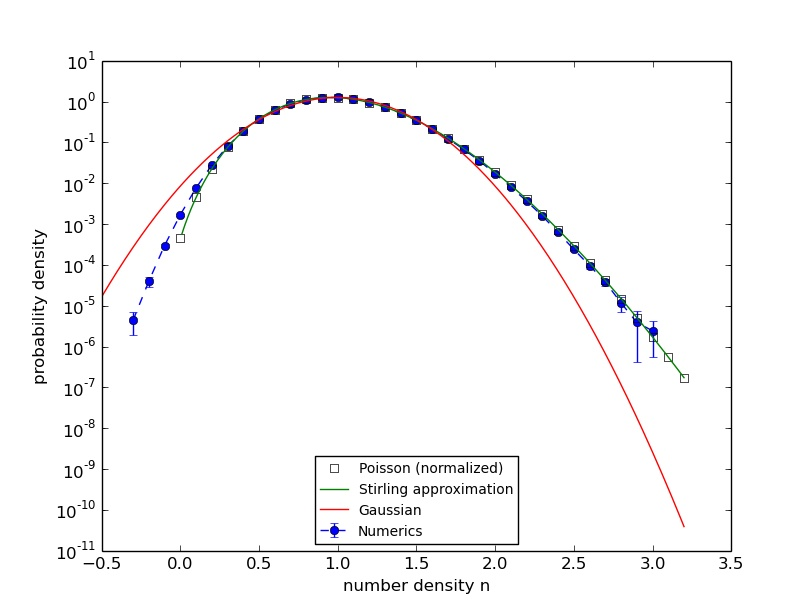
\includegraphics[width=0.5\linewidth,height=1.9in]{fig1/diff_dt0.25_hist_mid1.jpg}
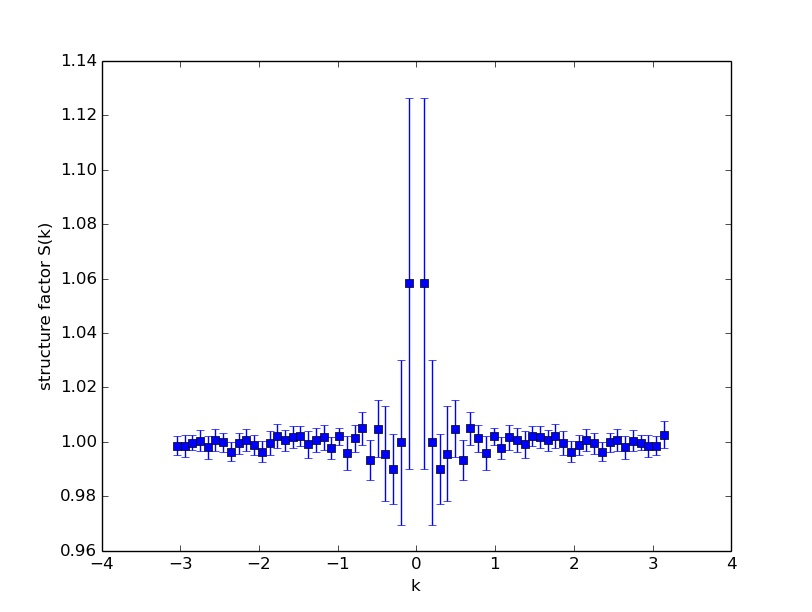
\includegraphics[width=0.5\linewidth,height=1.9in]{fig1/diff_dt0.25_Sk_mid1.jpg}
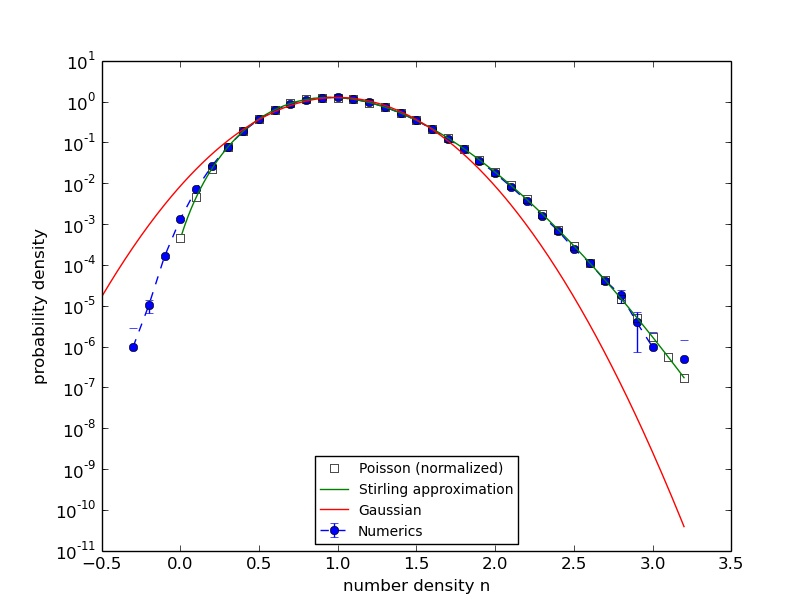
\includegraphics[width=0.5\linewidth,height=1.9in]{fig1/diff_dt0.25_hist_mid2.jpg}
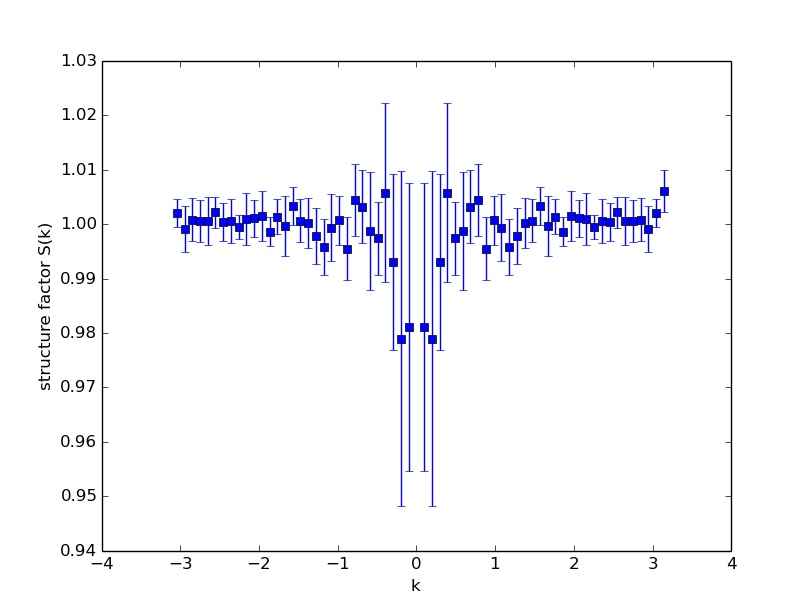
\includegraphics[width=0.5\linewidth,height=1.9in]{fig1/diff_dt0.25_Sk_mid2.jpg}
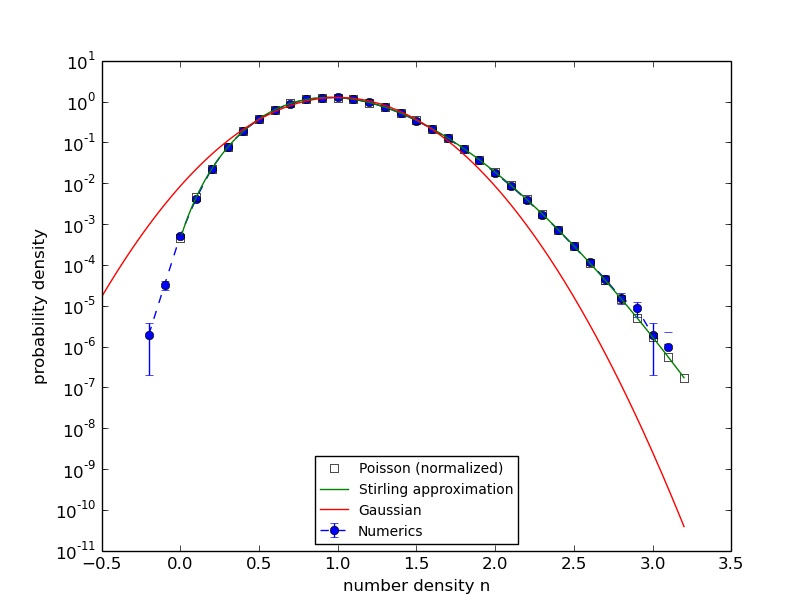
\includegraphics[width=0.5\linewidth,height=1.9in]{fig1/diff_dt0.25_hist_mid3.jpg}
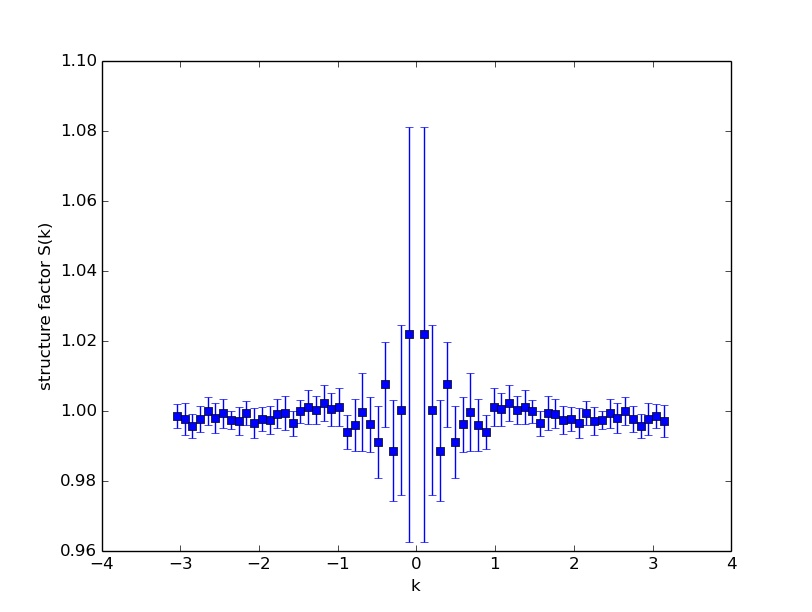
\includegraphics[width=0.5\linewidth,height=1.9in]{fig1/diff_dt0.25_Sk_mid3.jpg}
\caption{\label{fig_diff_dt0.25_mid_type}[Diffusion-only case with $\Delta t=0.25$] Results of $\rho(n)$ (left column) and $S(k)$ (right column) for \texttt{midpoint\_stoch\_flux\_type=1} (top row), \texttt{midpoint\_stoch\_flux\_type=2} (middle row), and \texttt{midpoint\_stoch\_flux\_type=3} (bottom row).
}
\end{figure}

\begin{figure}
\begin{center}
\framebox[1.2\width]{Diffusion-only, $\Delta t=1$}
\end{center}
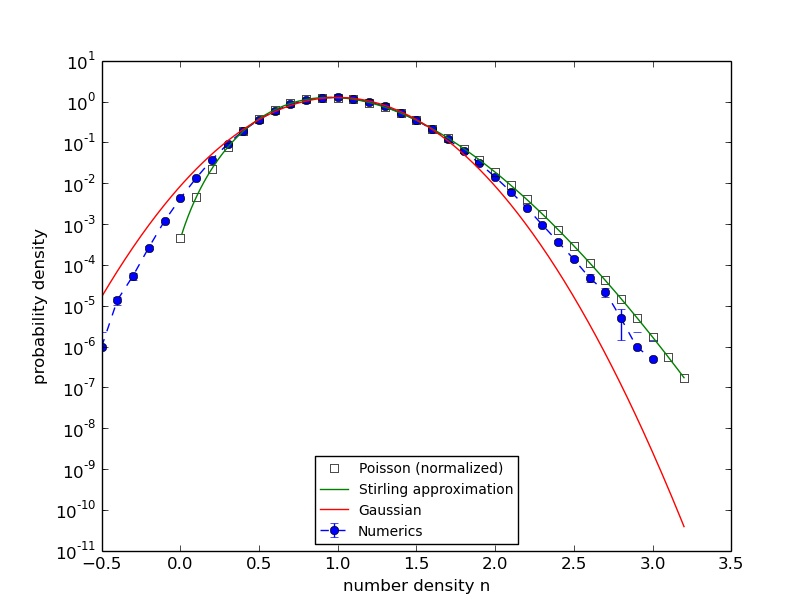
\includegraphics[width=0.5\linewidth,height=1.9in]{fig1/diff_dt1_hist_mid1.jpg}
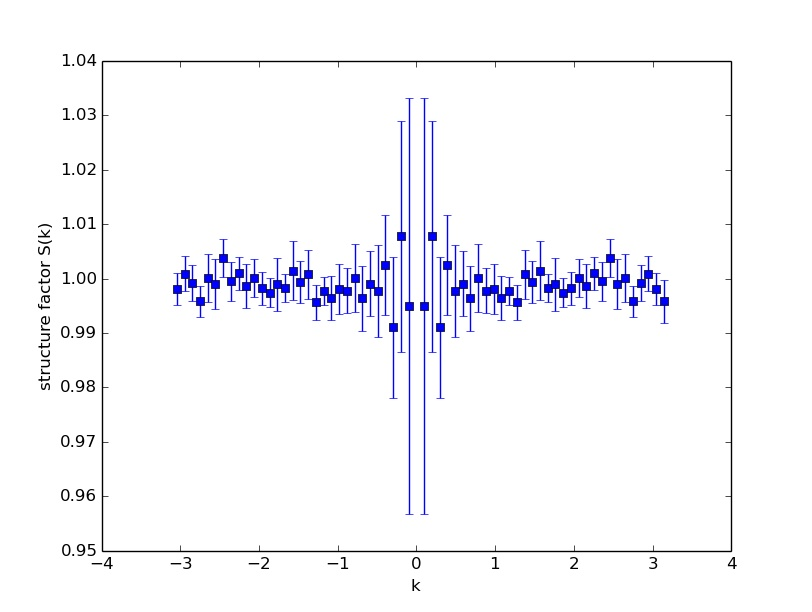
\includegraphics[width=0.5\linewidth,height=1.9in]{fig1/diff_dt1_Sk_mid1.jpg}
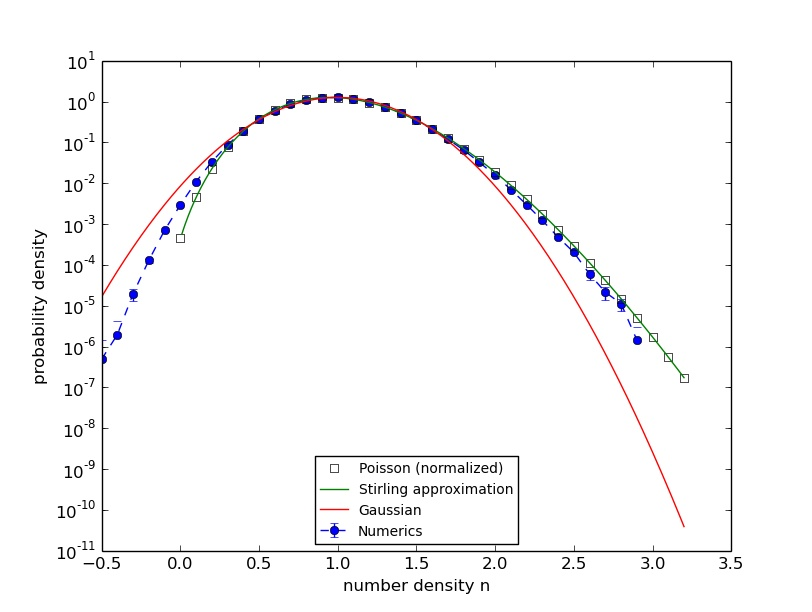
\includegraphics[width=0.5\linewidth,height=1.9in]{fig1/diff_dt1_hist_mid2.jpg}
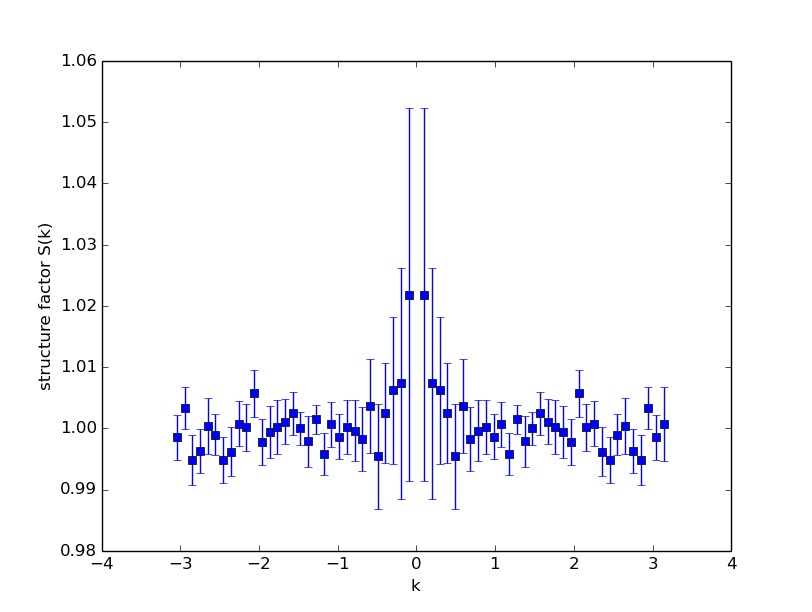
\includegraphics[width=0.5\linewidth,height=1.9in]{fig1/diff_dt1_Sk_mid2.jpg}
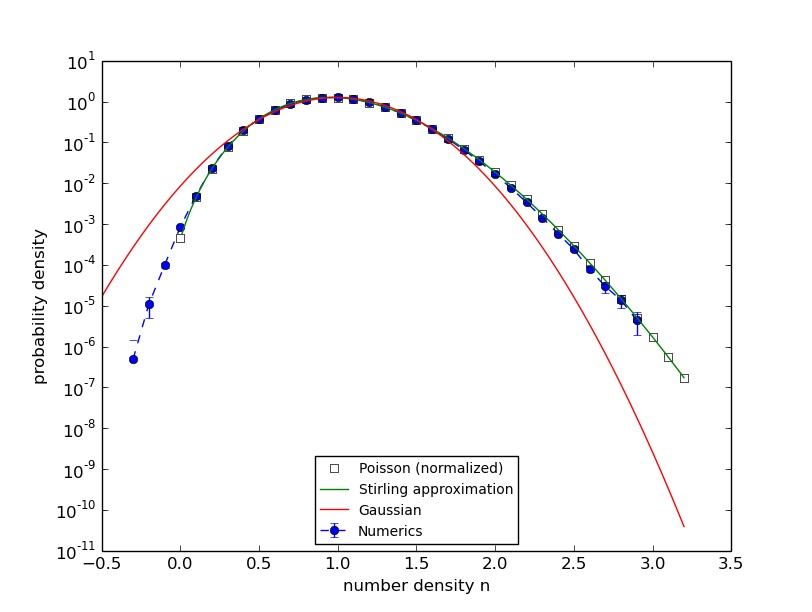
\includegraphics[width=0.5\linewidth,height=1.9in]{fig1/diff_dt1_hist_mid3.jpg}
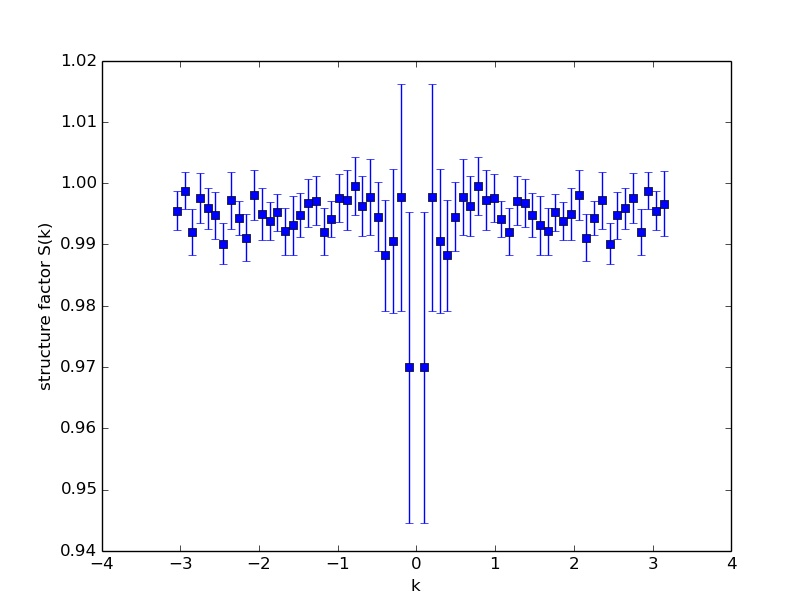
\includegraphics[width=0.5\linewidth,height=1.9in]{fig1/diff_dt1_Sk_mid3.jpg}
\caption{\label{fig_diff_dt1_mid_type}[Diffusion-only case with $\Delta t=1$] Results of $\rho(n)$ (left column) and $S(k)$ (right column) for \texttt{midpoint\_stoch\_flux\_type=1} (top row), \texttt{midpoint\_stoch\_flux\_type=2} (middle row), and \texttt{midpoint\_stoch\_flux\_type=3} (bottom row).
}
\end{figure}

\begin{figure}
\begin{center}
\framebox[1.2\width]{Diffusion-only, $\Delta t=2$}
\end{center}
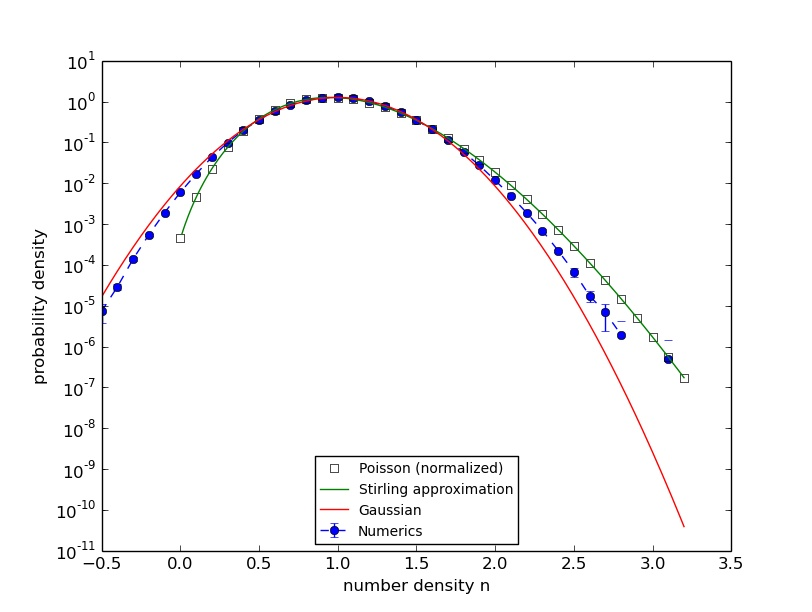
\includegraphics[width=0.5\linewidth,height=1.9in]{fig1/diff_dt2_hist_mid1.jpg}
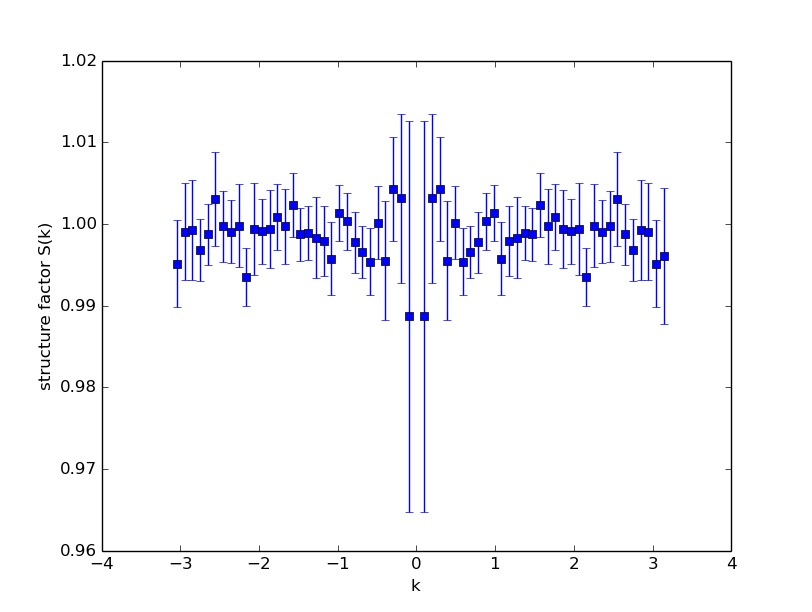
\includegraphics[width=0.5\linewidth,height=1.9in]{fig1/diff_dt2_Sk_mid1.jpg}
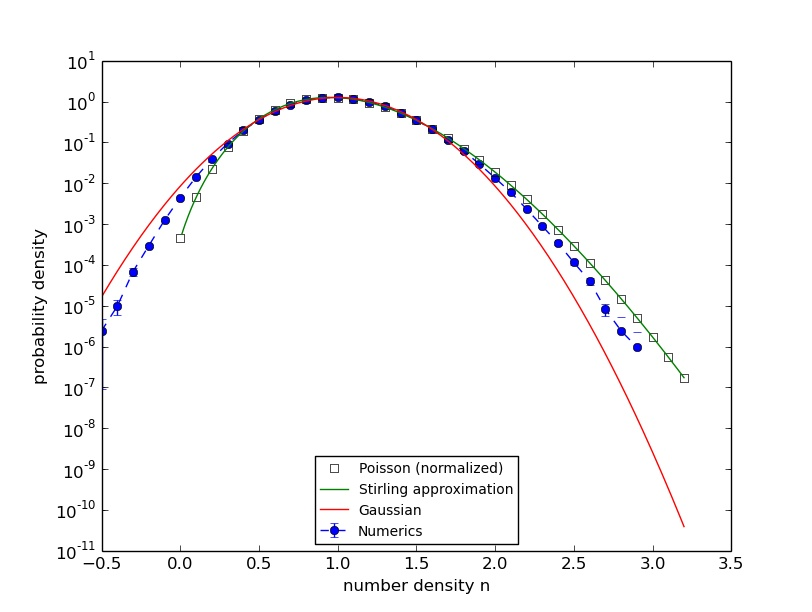
\includegraphics[width=0.5\linewidth,height=1.9in]{fig1/diff_dt2_hist_mid2.jpg}
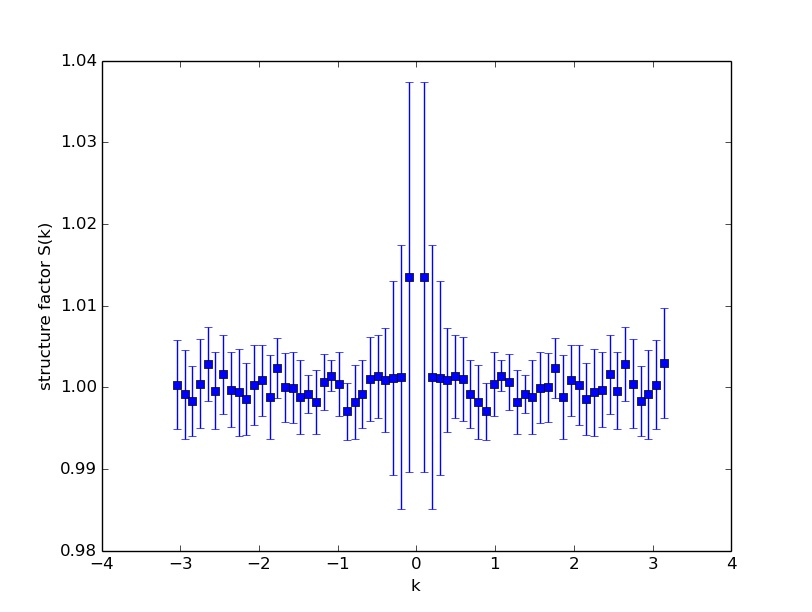
\includegraphics[width=0.5\linewidth,height=1.9in]{fig1/diff_dt2_Sk_mid2.jpg}
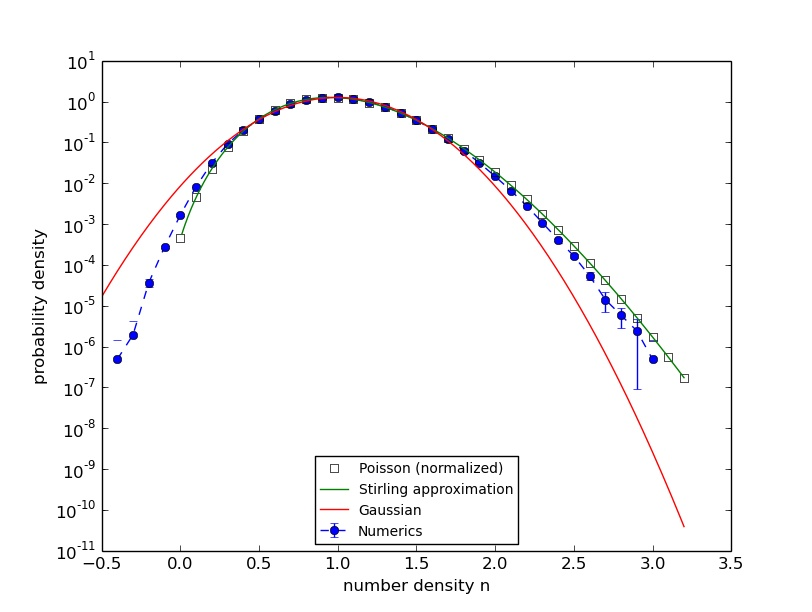
\includegraphics[width=0.5\linewidth,height=1.9in]{fig1/diff_dt2_hist_mid3.jpg}
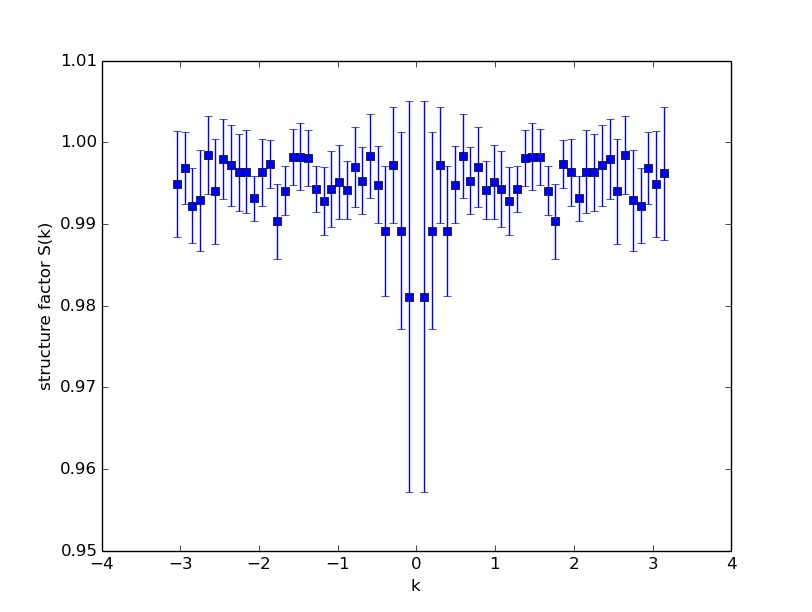
\includegraphics[width=0.5\linewidth,height=1.9in]{fig1/diff_dt2_Sk_mid3.jpg}
\caption{\label{fig_diff_dt2_mid_type}[Diffusion-only case with $\Delta t=2$] Results of $\rho(n)$ (left column) and $S(k)$ (right column) for \texttt{midpoint\_stoch\_flux\_type=1} (top row), \texttt{midpoint\_stoch\_flux\_type=2} (middle row), and \texttt{midpoint\_stoch\_flux\_type=3} (bottom row).
}
\end{figure}

\begin{figure}
\begin{center}
\framebox[1.2\width]{Reaction-diffusion, $\Delta t=0.25$}
\end{center}
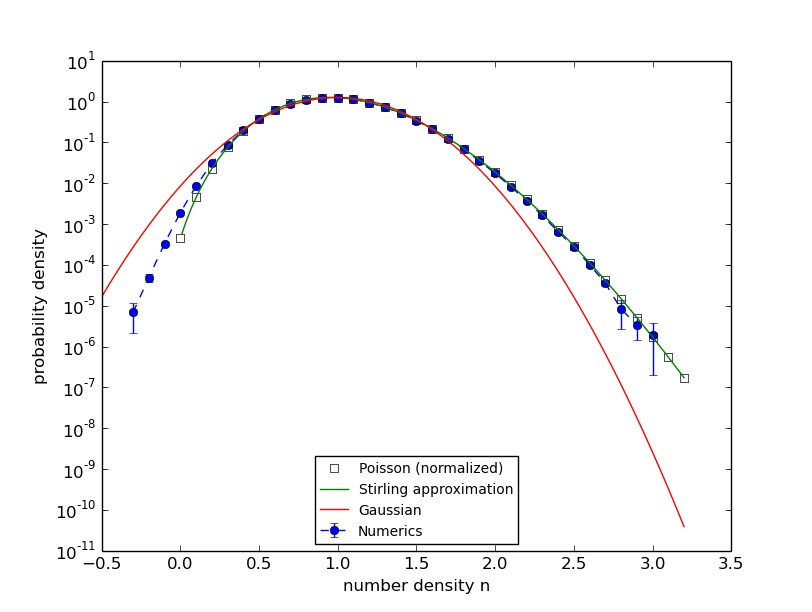
\includegraphics[width=0.5\linewidth,height=1.9in]{fig1/react_dt0.25_hist_mid1.jpg}
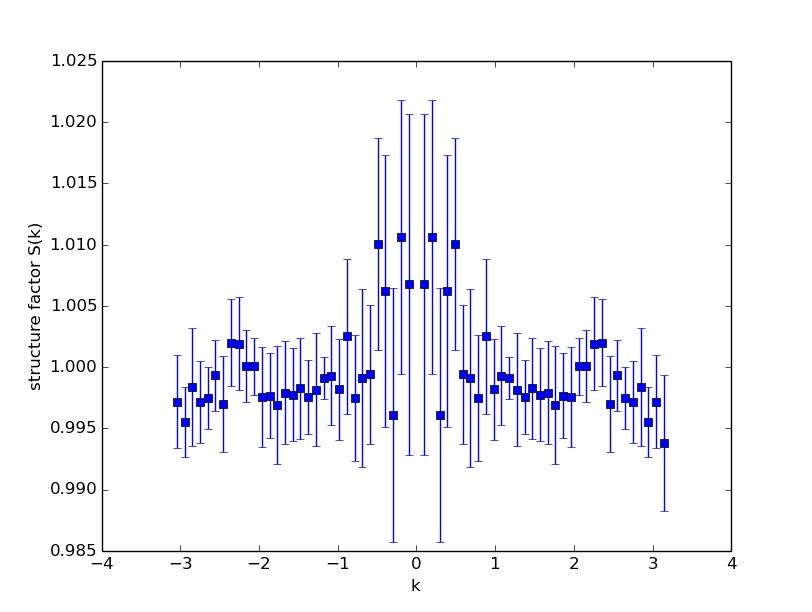
\includegraphics[width=0.5\linewidth,height=1.9in]{fig1/react_dt0.25_Sk_mid1.jpg}
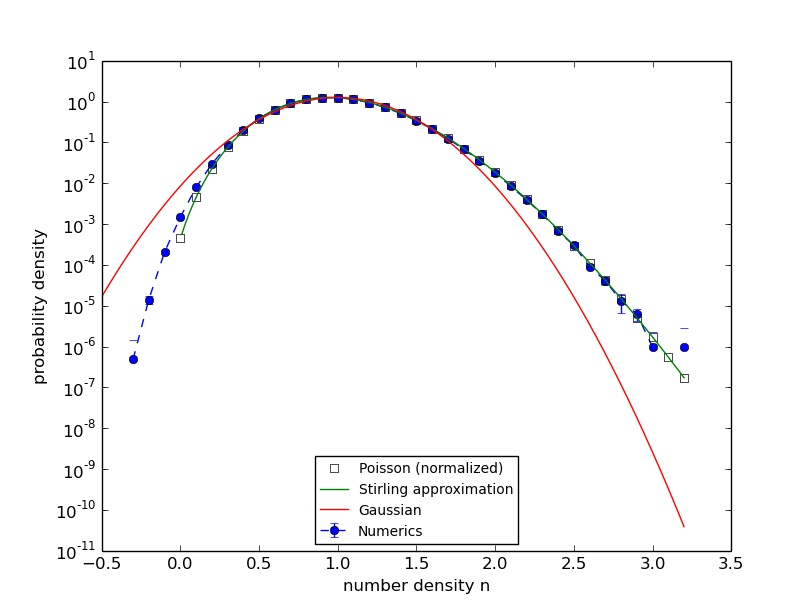
\includegraphics[width=0.5\linewidth,height=1.9in]{fig1/react_dt0.25_hist_mid2.jpg}
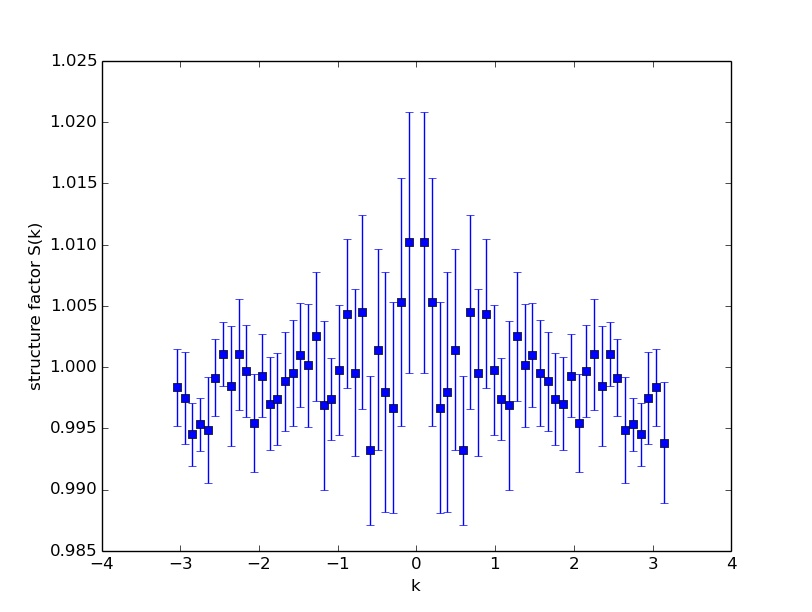
\includegraphics[width=0.5\linewidth,height=1.9in]{fig1/react_dt0.25_Sk_mid2.jpg}
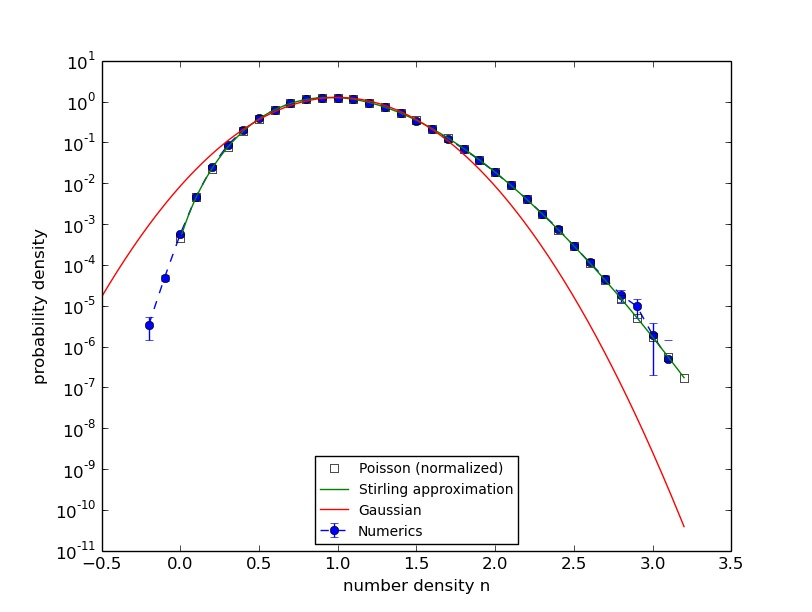
\includegraphics[width=0.5\linewidth,height=1.9in]{fig1/react_dt0.25_hist_mid3.jpg}
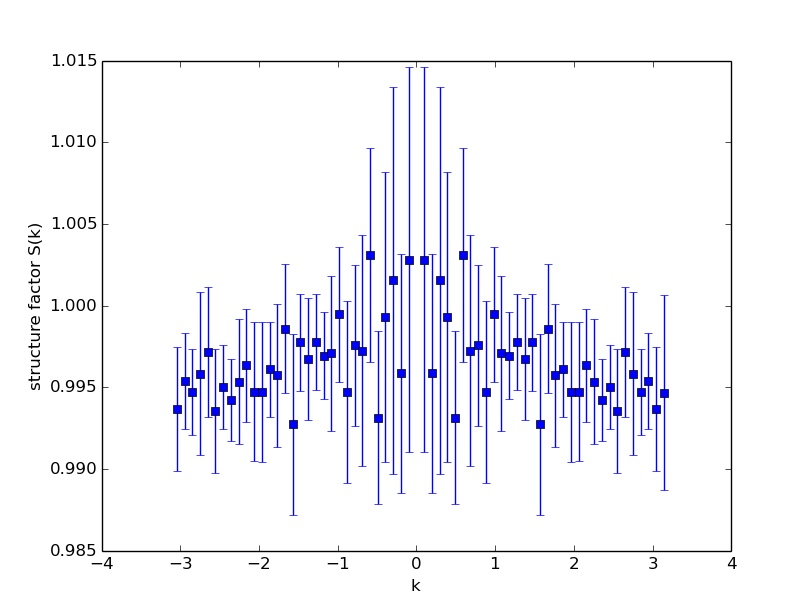
\includegraphics[width=0.5\linewidth,height=1.9in]{fig1/react_dt0.25_Sk_mid3.jpg}
\caption{\label{fig_react_dt0.25_mid_type}[Reaction-diffusion case with $\Delta t=0.25$] Results of $\rho(n)$ (left column) and $S(k)$ (right column) for \texttt{midpoint\_stoch\_flux\_type=1} (top row), \texttt{midpoint\_stoch\_flux\_type=2} (middle row), and \texttt{midpoint\_stoch\_flux\_type=3} (bottom row).
}
\end{figure}

\begin{figure}
\begin{center}
\framebox[1.2\width]{Reaction-diffusion, $\Delta t=1$}
\end{center}
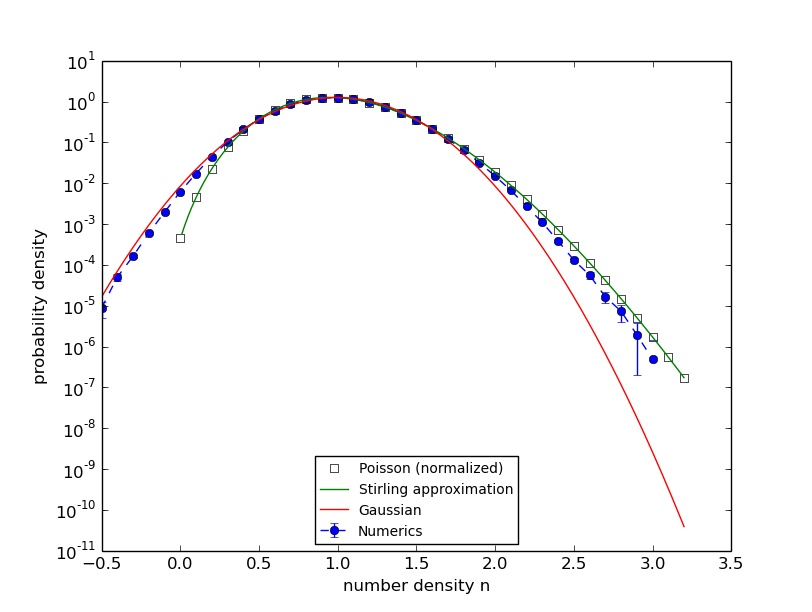
\includegraphics[width=0.5\linewidth,height=1.9in]{fig1/react_dt1_hist_mid1.jpg}
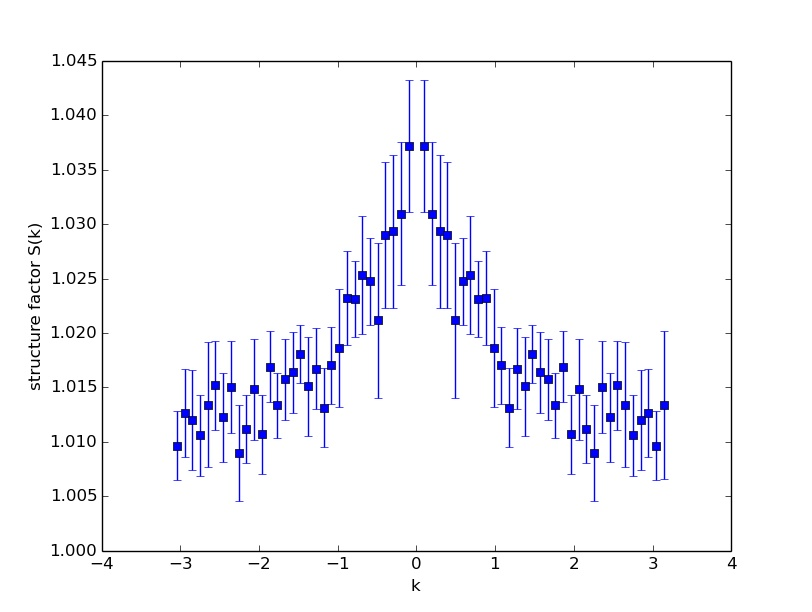
\includegraphics[width=0.5\linewidth,height=1.9in]{fig1/react_dt1_Sk_mid1.jpg}
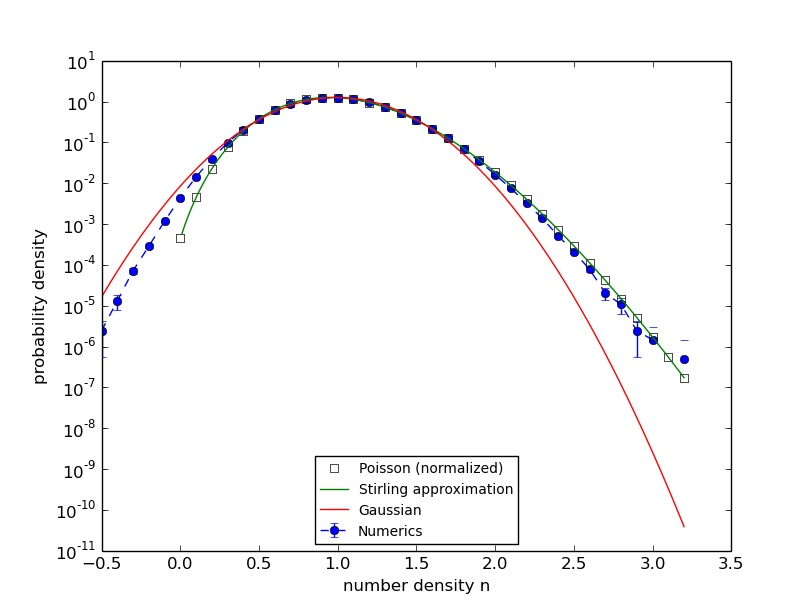
\includegraphics[width=0.5\linewidth,height=1.9in]{fig1/react_dt1_hist_mid2.jpg}
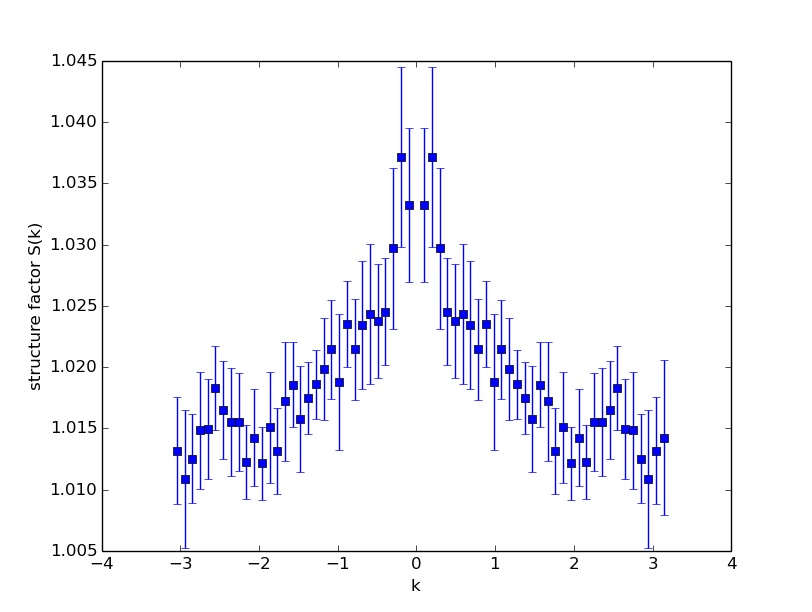
\includegraphics[width=0.5\linewidth,height=1.9in]{fig1/react_dt1_Sk_mid2.jpg}
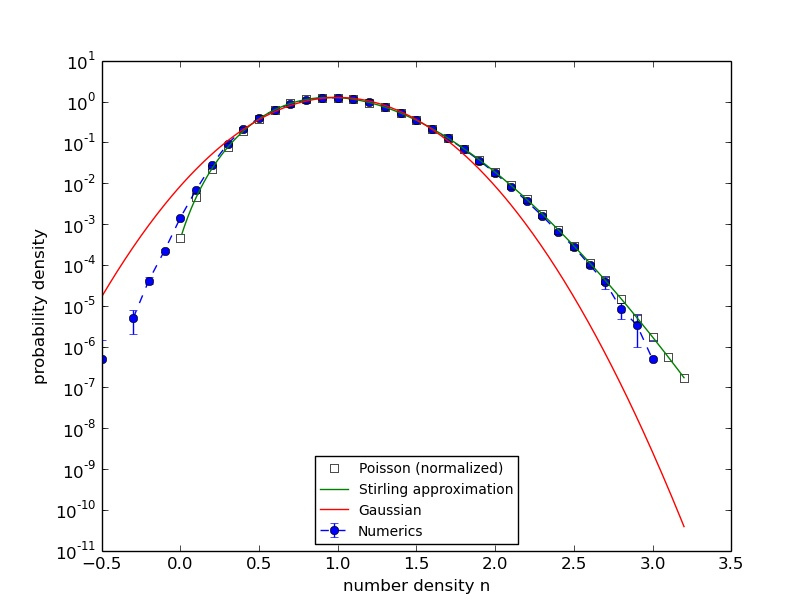
\includegraphics[width=0.5\linewidth,height=1.9in]{fig1/react_dt1_hist_mid3.jpg}
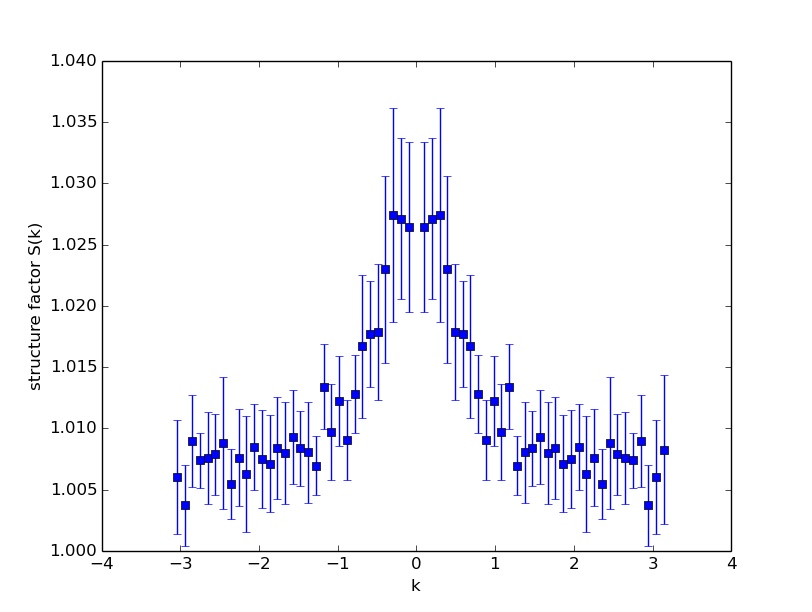
\includegraphics[width=0.5\linewidth,height=1.9in]{fig1/react_dt1_Sk_mid3.jpg}
\caption{\label{fig_react_dt1_mid_type}[Reaction-diffusion case with $\Delta t=1$] Results of $\rho(n)$ (left column) and $S(k)$ (right column) for \texttt{midpoint\_stoch\_flux\_type=1} (top row), \texttt{midpoint\_stoch\_flux\_type=2} (middle row), and \texttt{midpoint\_stoch\_flux\_type=3} (bottom row).
}
\end{figure}

\begin{figure}
\begin{center}
\framebox[1.2\width]{Reaction-diffusion, $\Delta t=2$}
\end{center}
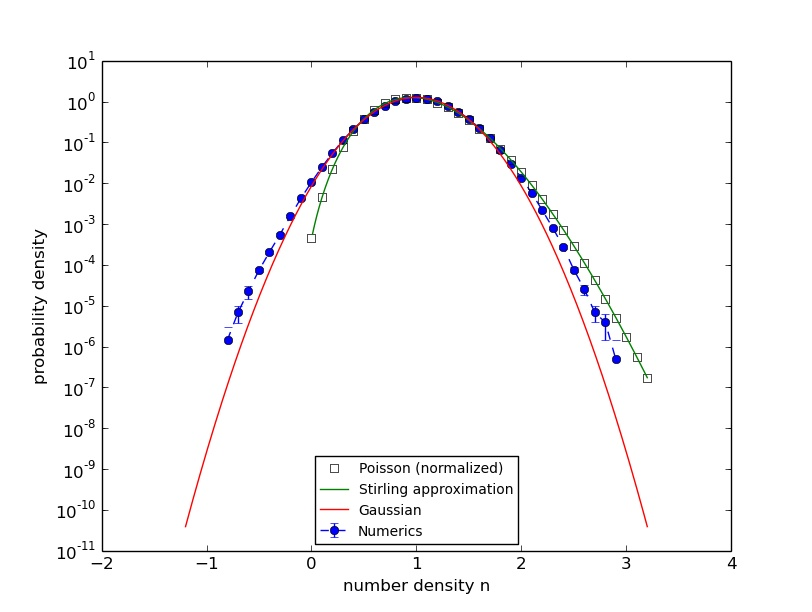
\includegraphics[width=0.5\linewidth,height=1.9in]{fig1/react_dt2_hist_mid1.jpg}
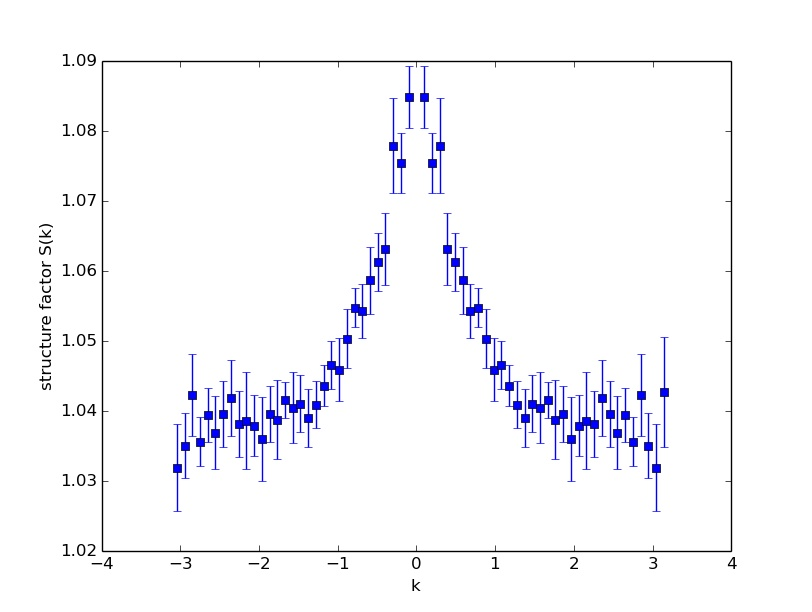
\includegraphics[width=0.5\linewidth,height=1.9in]{fig1/react_dt2_Sk_mid1.jpg}
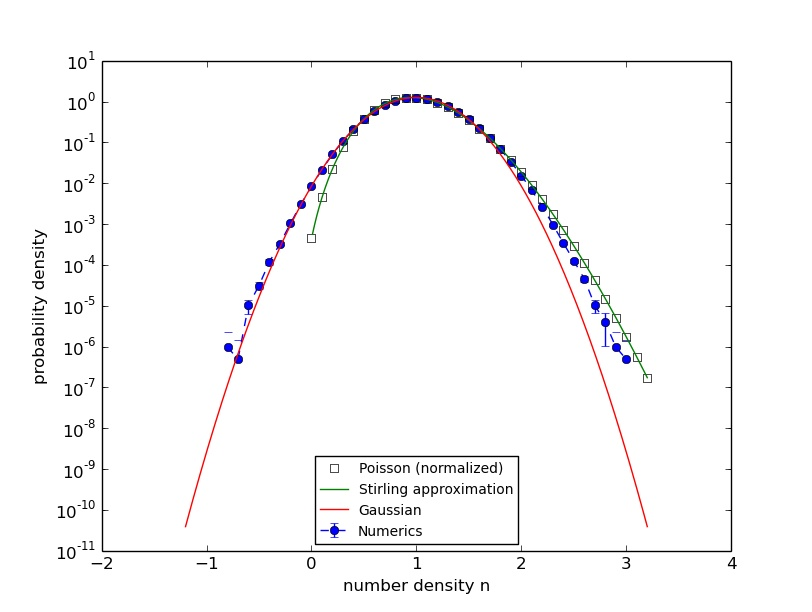
\includegraphics[width=0.5\linewidth,height=1.9in]{fig1/react_dt2_hist_mid2.jpg}
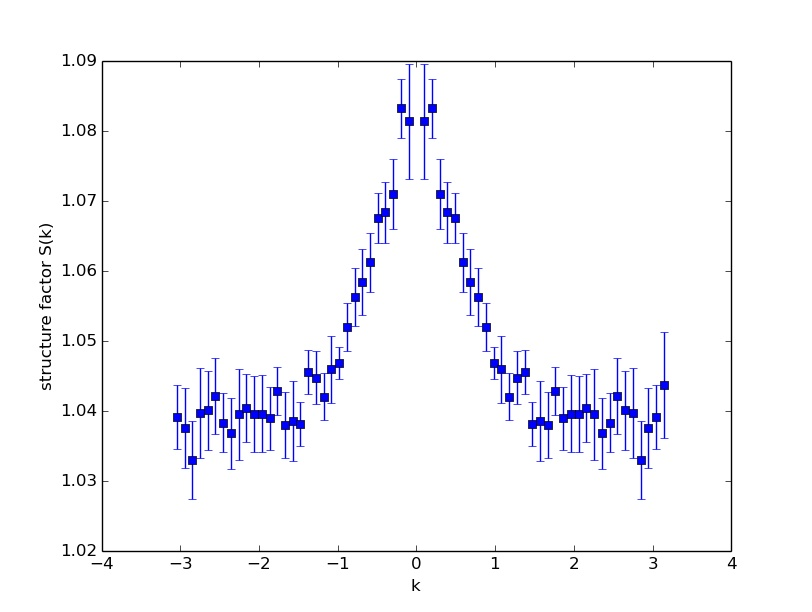
\includegraphics[width=0.5\linewidth,height=1.9in]{fig1/react_dt2_Sk_mid2.jpg}
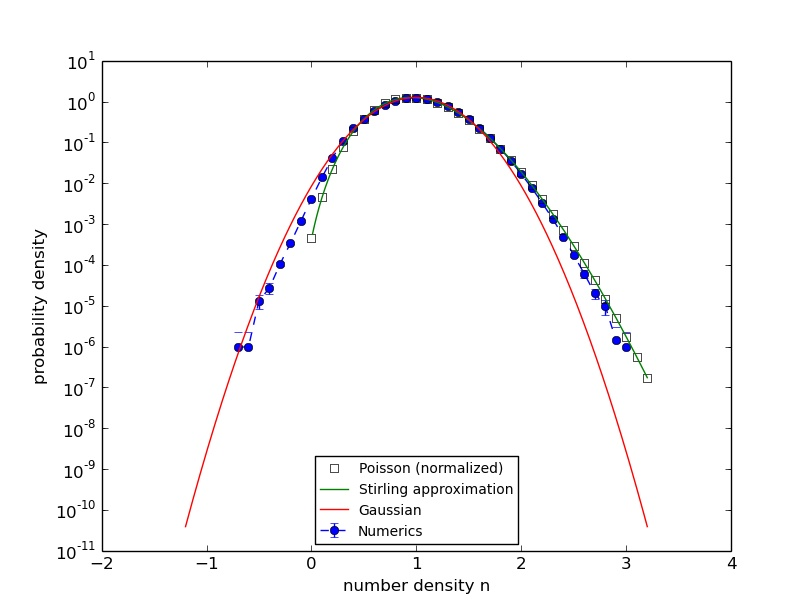
\includegraphics[width=0.5\linewidth,height=1.9in]{fig1/react_dt2_hist_mid3.jpg}
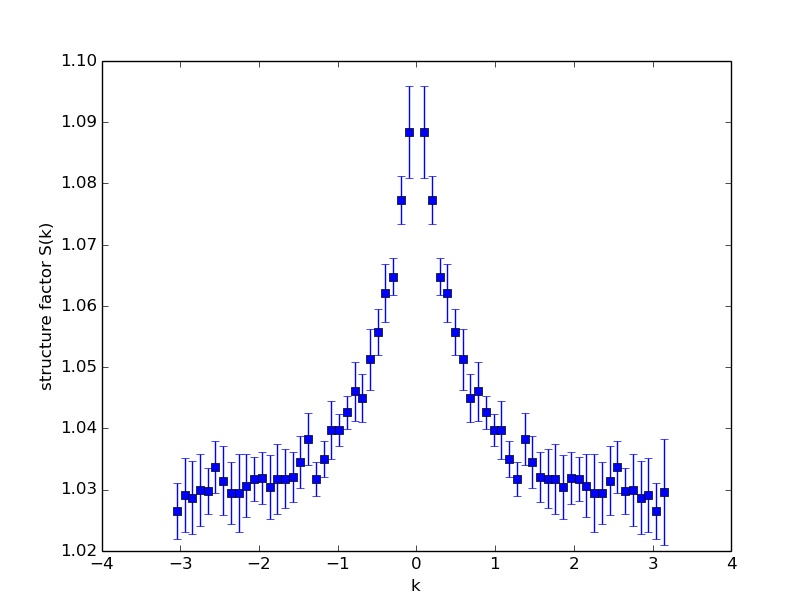
\includegraphics[width=0.5\linewidth,height=1.9in]{fig1/react_dt2_Sk_mid3.jpg}
\caption{\label{fig_react_dt2_mid_type}[Reaction-diffusion case with $\Delta t=2$] Results of $\rho(n)$ (left column) and $S(k)$ (right column) for \texttt{midpoint\_stoch\_flux\_type=1} (top row), \texttt{midpoint\_stoch\_flux\_type=2} (middle row), and \texttt{midpoint\_stoch\_flux\_type=3} (bottom row).
}
\end{figure}

Figures~\ref{fig_diff_dt0.25_mid_type}, \ref{fig_diff_dt1_mid_type}, and \ref{fig_diff_dt2_mid_type} show numerical results of $\rho(n)$ and $S(k)$ for the diffusion-only case with $\Delta t=0.25$, 1, and 2, respectively.
Figures~\ref{fig_react_dt0.25_mid_type}, \ref{fig_react_dt1_mid_type}, and \ref{fig_react_dt2_mid_type} show numerical results of $\rho(n)$ and $S(k)$ for the reaction-diffusion case with $\Delta t=0.25$, 1, and 2, respectively.

The statistics of cell number density $n$ for $\Delta t=0.25$, 1, and 2 are as follows. Note that the mean values of $n$ are not shown for the diffusion-only case; since the total mass is conserved in the numerical scheme, they are exactly $n_\mathrm{eq}$.
\begin{center}
{\tabulinesep=1.2mm
($\Delta t=0.25$)\\
\vspace{1mm}
\begin{tabu}{|c|c|c|c|}
\hline
\multirow{2}{*}{\texttt{midpoint\_stoch\_flux\_type}} & Diffusion-only & \multicolumn{2}{c|}{Reaction-diffusion} \\
\cline{2-4}
 & $\mathrm{Var}[n]$ (SE) & $\mathrm{Mean}[n]$ (SE) & $\mathrm{Var}[n]$ (SE) \\
\hline
\texttt{1} & 0.09856 ($1.2\times10^{-4}$) & 0.9956 ($2\times10^{-4}$) & 0.10001 ($6\times10^{-5}$) \\
\hline
\texttt{2} & 0.09834 ($0.9\times10^{-4}$) & 0.9949 ($4\times10^{-4}$) & 0.09991 ($7\times10^{-5}$) \\
\hline
\texttt{3} & 0.09833 ($1.0\times10^{-4}$) & 0.9952 ($3\times10^{-4}$) & 0.09966 ($6\times10^{-5}$) \\
\hline
\end{tabu}
}
\end{center}
\begin{center}
{\tabulinesep=1.2mm
($\Delta t=1$)\\
\vspace{1mm}
\begin{tabu}{|c|c|c|c|}
\hline
\multirow{2}{*}{\texttt{midpoint\_stoch\_flux\_type}} & Diffusion-only & \multicolumn{2}{c|}{Reaction-diffusion} \\
\cline{2-4}
 & $\mathrm{Var}[n]$ (SE) & $\mathrm{Mean}[n]$ (SE) & $\mathrm{Var}[n]$ (SE) \\
\hline
\texttt{1} & 0.09832 ($0.7\times10^{-4}$) & 0.9972 ($2\times10^{-4}$) & 0.10178 ($4\times10^{-5}$) \\
\hline
\texttt{2} & 0.09850 ($0.7\times10^{-4}$) & 0.9976 ($2\times10^{-4}$) & 0.10192 ($4\times10^{-5}$) \\
\hline
\texttt{3} & 0.09787 ($0.8\times10^{-4}$) & 0.9973 ($2\times10^{-4}$) & 0.10117 ($4\times10^{-5}$) \\
\hline
\end{tabu}
}
\end{center}
\begin{center}
{\tabulinesep=1.2mm
($\Delta t=2$)\\
\vspace{1mm}
\begin{tabu}{|c|c|c|c|}
\hline
\multirow{2}{*}{\texttt{midpoint\_stoch\_flux\_type}} & Diffusion-only & \multicolumn{2}{c|}{Reaction-diffusion} \\
\cline{2-4}
 & $\mathrm{Var}[n]$ (SE) & $\mathrm{Mean}[n]$ (SE) & $\mathrm{Var}[n]$ (SE) \\
\hline
\texttt{1} & 0.09830 ($0.6\times10^{-4}$) & 1.0034 ($2\times10^{-4}$) & 0.10475 ($4\times10^{-5}$) \\
\hline
\texttt{2} & 0.09849 ($0.8\times10^{-4}$) & 1.0032 ($2\times10^{-4}$) & 0.10484 ($5\times10^{-5}$) \\
\hline
\texttt{3} & 0.09792 ($0.7\times10^{-4}$) & 1.0028 ($2\times10^{-4}$) & 0.10406 ($5\times10^{-5}$) \\
\hline
\end{tabu}
}
\end{center}

Results for $\Delta t=0.25$ demonstrate the case that the time step is quite small and the scheme works well.
It is noted, however, that this time step is so large for the explicit scheme that the latter scheme does not work very well (see Appendix~B). 
Results for $\Delta t=1$ demonstrate the case that the time step is quite large but the scheme still works well.
On the other hand, results for $\Delta t=2$ demonstrate the case that the time step is so large that the scheme does not work very well.

For the diffusion-only case, changes in $\rho(n)$ are more noticeable than $S(k)$.
$S(k)$ maintains the flat shape having values around $n_\mathrm{eq}$ even for $\Delta t=2$ and the difference among different \texttt{midpoint\_stoch\_flux\_type} option values is not so obvious.
On the other hand, \texttt{midpoint\_stoch\_flux\_type=3} exhibits a much more favorable distribution $\rho(n)$ than the other option values for $\Delta t=0.25$ and 1 (i.e., smaller chances of negative densities and closer to the Poisson distribution), but for $\Delta t=2$ this option also shows significant deviation from the Poisson distribution. 

For the reaction-diffusion case, changes in $\rho(n)$ and $S(k)$ are noticeable.
Although chances of negative densities are increased by reaction, overall trends are rather similar to the diffusion-only case.
On the other hand, as $\Delta t$ becomes large, $S(k)$ is no more flat and has a peak around $k=0$.
This behavior is expected from the linearized equation analysis.
In other words, even in the equilibrium monomodal case, the structure factor obtained from the scheme is not flat.
However, $S(k)$ values around $k=0$ is much higher than the theoretical values (1.001 for $\Delta t=1$ and 1.012 for $\Delta t=2$).
Since the linear approximation is not valid for the small-number-of-particles-in-a-cell case, this is not contradictory.
The difference among different option values is somewhat noticeable but it is not so clear to determine the best option value from $S(k)$.

\subsection*{\textbf{Best option value for \texttt{midpoint\_stoch\_flux\_type}}}

\texttt{midpoint\_stoch\_flux\_type=3} ($n_s^\bullet=\left[2n_s^{k+\myhalf}-n_s^k\right]^+$)

\clearpage

\subsection*{Appendix A.~Small Time Step Results for Different \texttt{avg\_type} and Multinomial Diffusion Method}

\begin{figure}
\begin{center}
\framebox[1.2\width]{Diffusion-only, $\Delta t=0.01$}
\end{center}
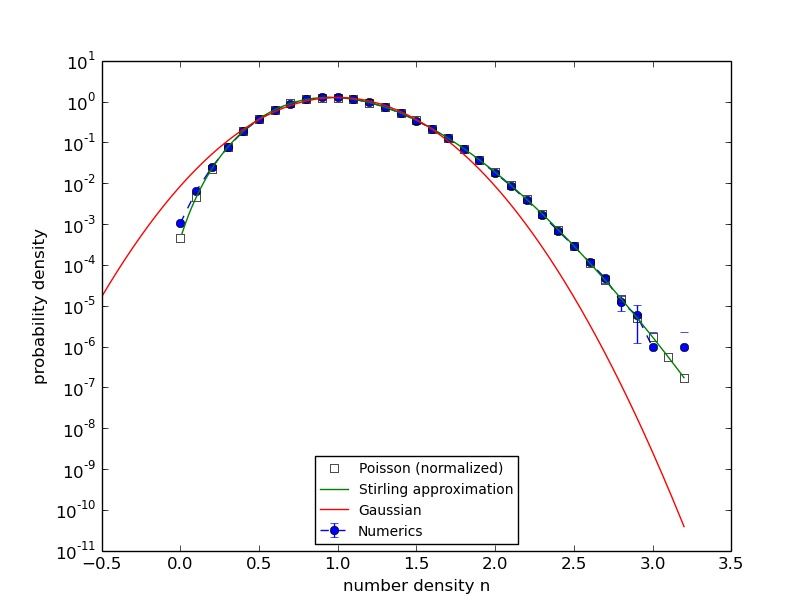
\includegraphics[width=0.5\linewidth,height=1.9in]{fig1/appendix_dt0.01_diff_hist_avg1.jpg}
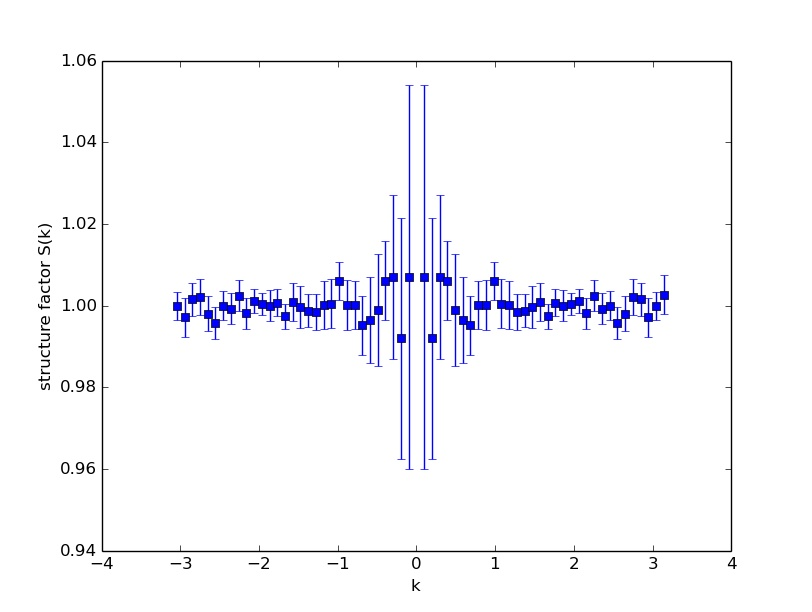
\includegraphics[width=0.5\linewidth,height=1.9in]{fig1/appendix_dt0.01_diff_Sk_avg1.jpg}
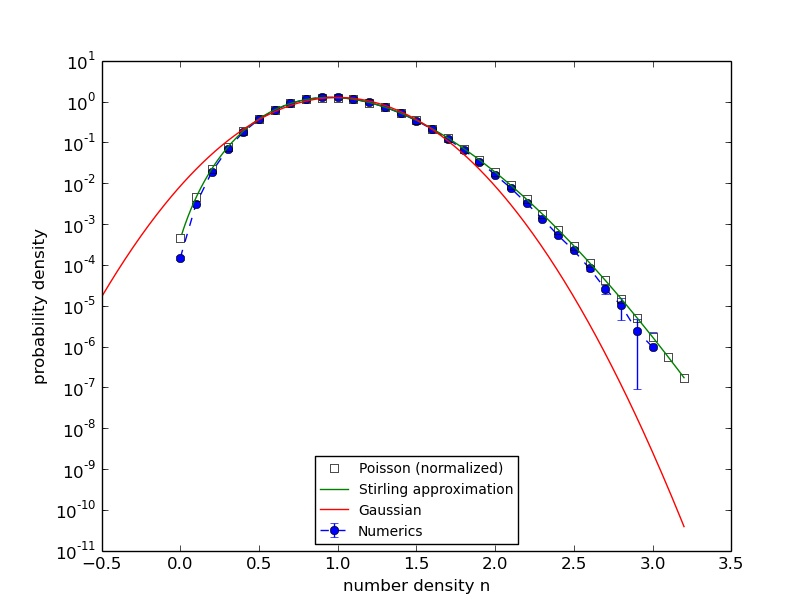
\includegraphics[width=0.5\linewidth,height=1.9in]{fig1/appendix_dt0.01_diff_hist_avg2.jpg}
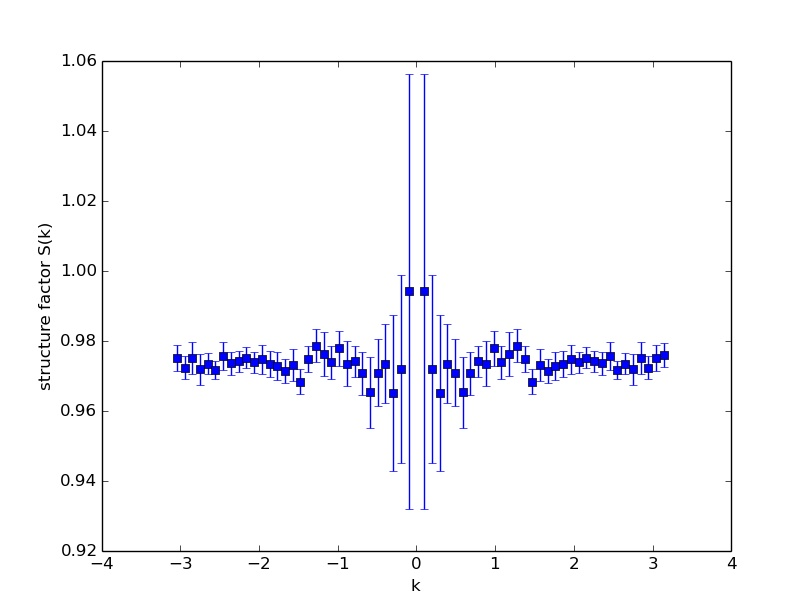
\includegraphics[width=0.5\linewidth,height=1.9in]{fig1/appendix_dt0.01_diff_Sk_avg2.jpg}
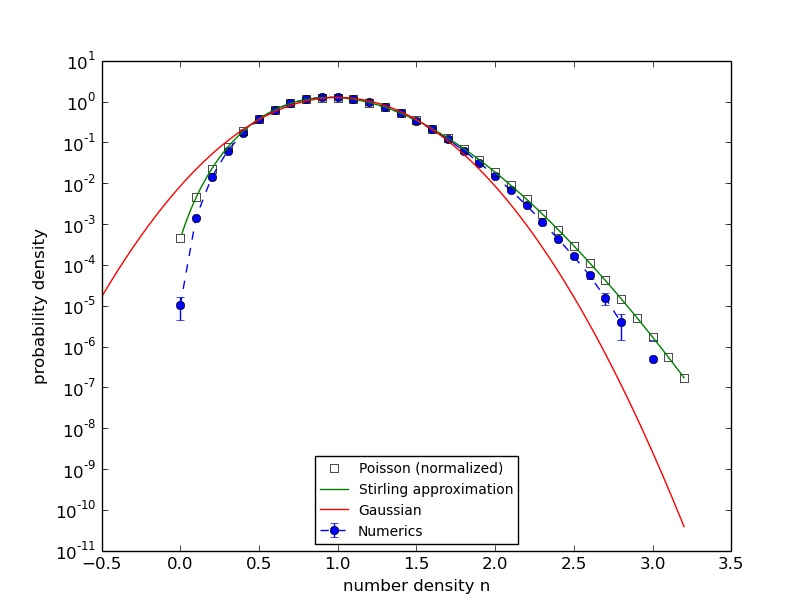
\includegraphics[width=0.5\linewidth,height=1.9in]{fig1/appendix_dt0.01_diff_hist_avg3.jpg}
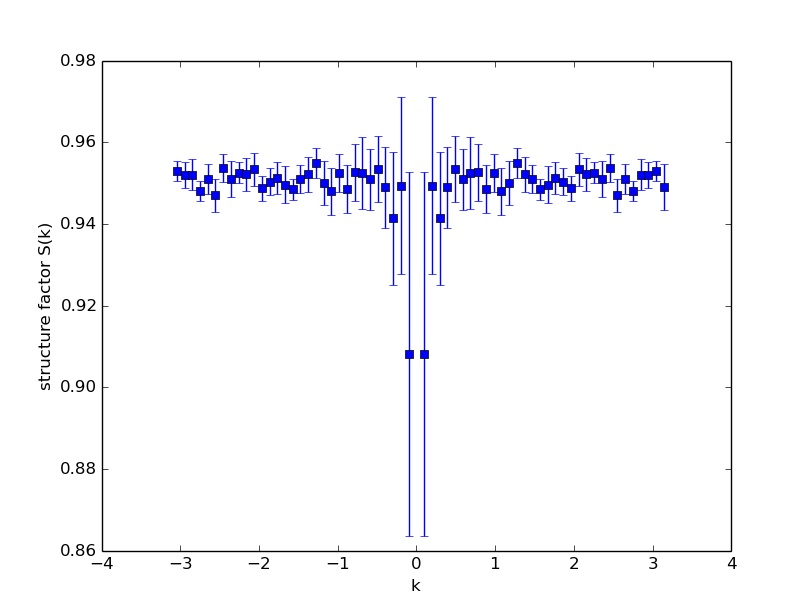
\includegraphics[width=0.5\linewidth,height=1.9in]{fig1/appendix_dt0.01_diff_Sk_avg3.jpg}
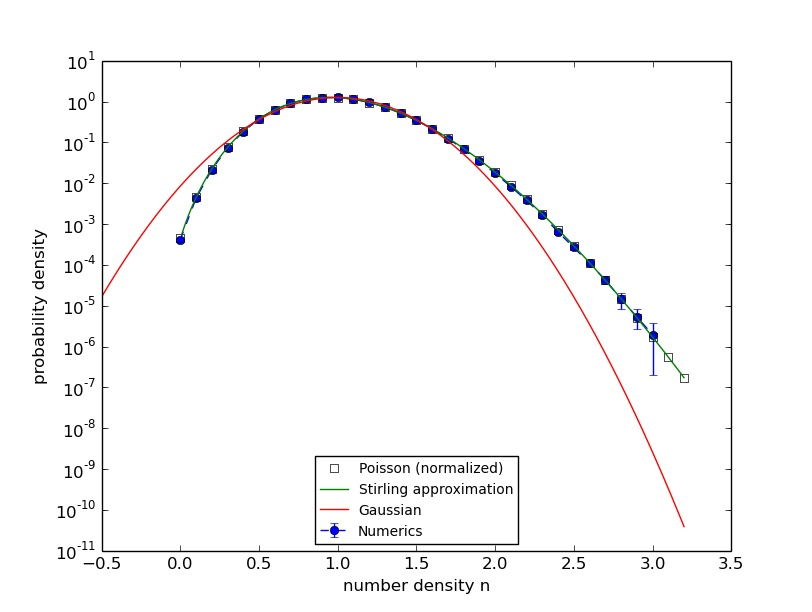
\includegraphics[width=0.5\linewidth,height=1.9in]{fig1/appendix_dt0.01_diff_hist_mn.jpg}
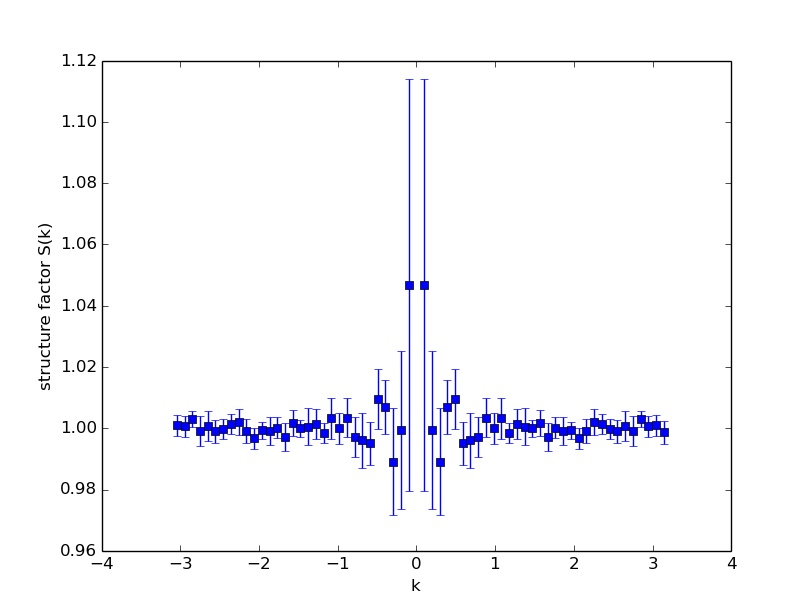
\includegraphics[width=0.5\linewidth,height=1.9in]{fig1/appendix_dt0.01_diff_Sk_mn.jpg}
\caption{\label{fig_appendix_diff_avg_type}[Diffusion-only case with $\Delta t=0.01$] Results of $\rho(n)$ (left column) and $S(k)$ (right column) for \texttt{avg\_type=1} (arithmetic mean, top row), \texttt{avg\_type=2} (geometric mean, upper-middle row), \texttt{avg\_type=3} (harmonic mean, lower-middle row), and the multinomial diffusion (bottom row).
}
\end{figure}

\begin{figure}
\begin{center}
\framebox[1.2\width]{Reaction-diffusion, $\Delta t=0.01$}
\end{center}
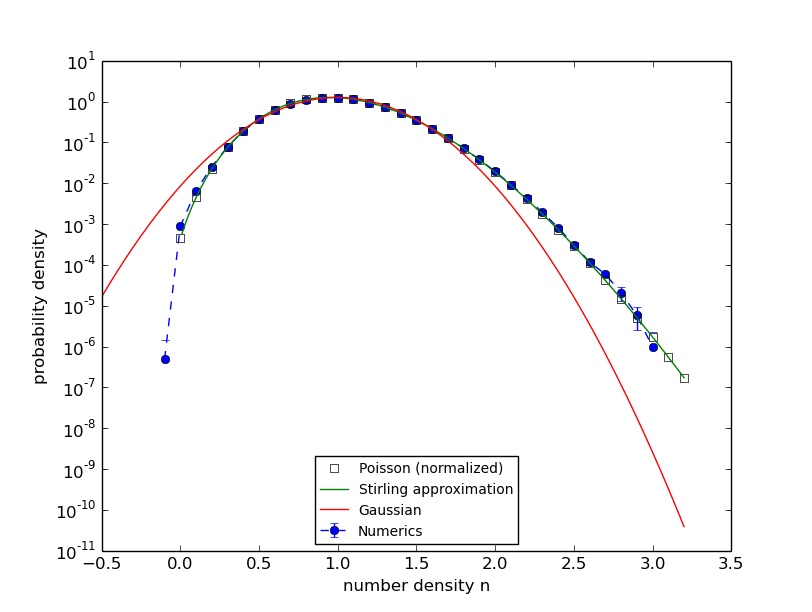
\includegraphics[width=0.5\linewidth,height=1.9in]{fig1/appendix_dt0.01_react_hist_avg1.jpg}
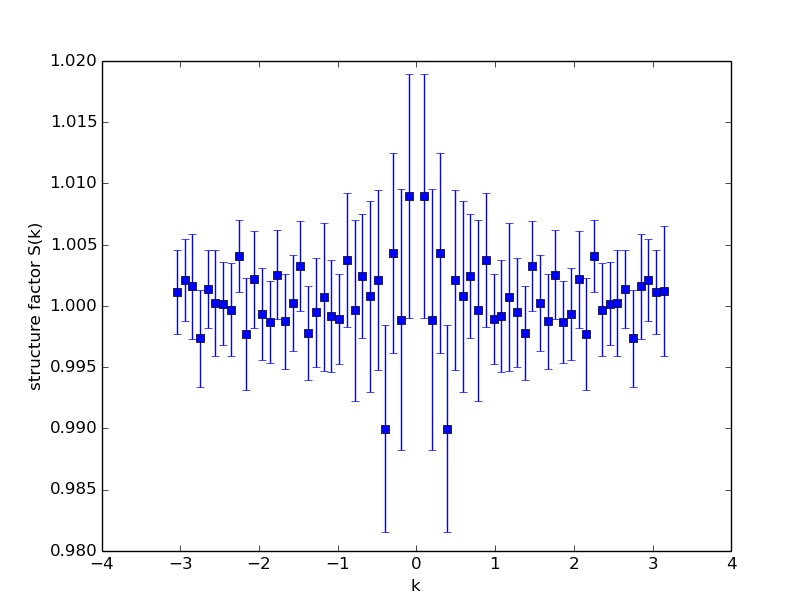
\includegraphics[width=0.5\linewidth,height=1.9in]{fig1/appendix_dt0.01_react_Sk_avg1.jpg}
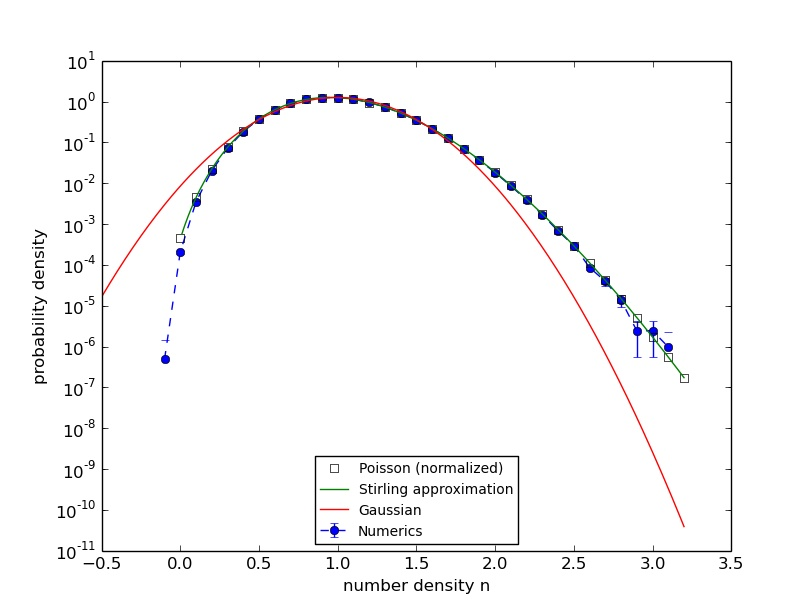
\includegraphics[width=0.5\linewidth,height=1.9in]{fig1/appendix_dt0.01_react_hist_avg2.jpg}
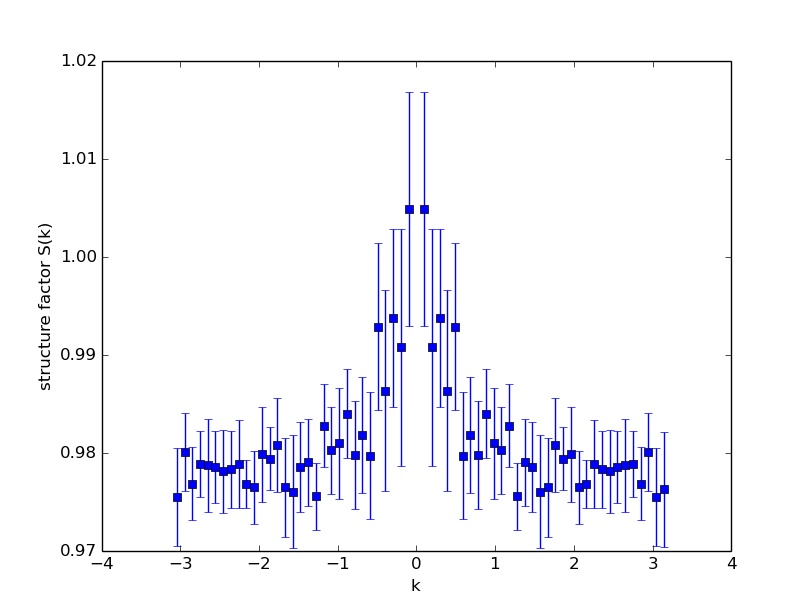
\includegraphics[width=0.5\linewidth,height=1.9in]{fig1/appendix_dt0.01_react_Sk_avg2.jpg}
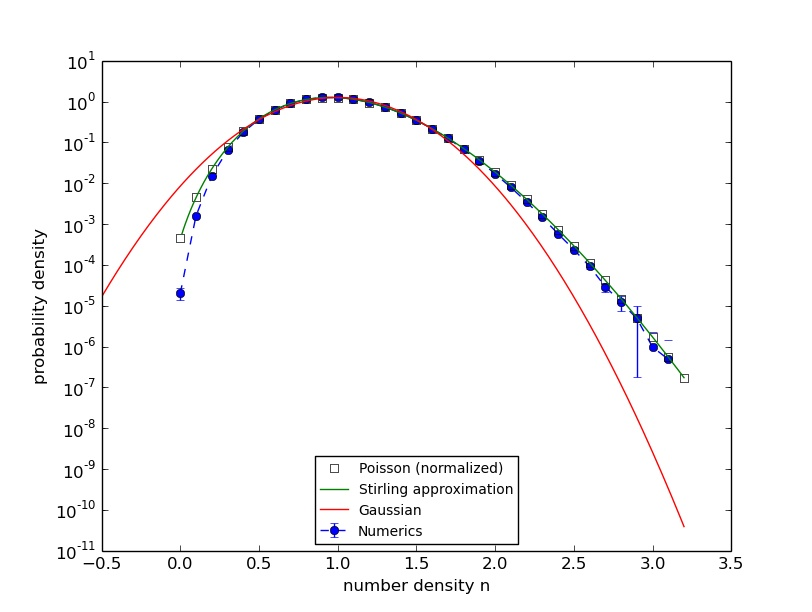
\includegraphics[width=0.5\linewidth,height=1.9in]{fig1/appendix_dt0.01_react_hist_avg3.jpg}
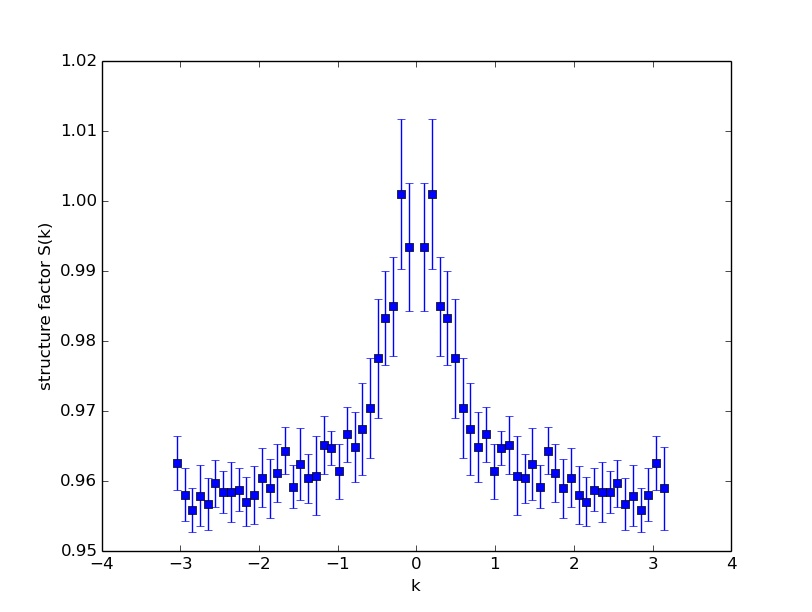
\includegraphics[width=0.5\linewidth,height=1.9in]{fig1/appendix_dt0.01_react_Sk_avg3.jpg}
\includegraphics[width=0.5\linewidth,height=1.9in]{fig1/appendix_dt0.01_react_hist_mn_ssa.jpg}
\includegraphics[width=0.5\linewidth,height=1.9in]{fig1/appendix_dt0.01_react_Sk_mn_ssa.jpg}
\caption{\label{fig_appendix_react_avg_type}[Reaction-diffusion case with $\Delta t=0.01$] Results of $\rho(n)$ (left column) and $S(k)$ (right column) for \texttt{avg\_type=1} (arithmetic mean, top row), \texttt{avg\_type=2} (geometric mean, upper-middle row), \texttt{avg\_type=3} (harmonic mean, lower-middle row), and the multinomial diffusion (bottom row).
}
\end{figure}

Figures~\ref{fig_appendix_diff_avg_type} and \ref{fig_appendix_react_avg_type} show numerical results for the diffusion-only and reaction-diffusion cases, respectively, which were obtained from the unsplitting explicit midpoint predictor-corrector (with \texttt{midpoint\_stoch\_flux\_type=3}) or the multinomial diffusion + SSA reaction scheme with small time step $\Delta t=0.01$.
Note that in \texttt{avg\_type=1} the smoothed Heaviside function $H_1(x)$ is applied.

The statistics of cell number density $n$ is as follows:
\begin{center}
{\tabulinesep=1.2mm
\begin{tabu}{|c|c|c|c|}
\hline
\multirow{2}{*}{\texttt{avg\_type}} & Diffusion-only & \multicolumn{2}{c|}{Reaction-diffusion} \\
\cline{2-4}
 & $\mathrm{Var}[n]$ (SE) & $\mathrm{Mean}[n]$ (SE) & $\mathrm{Var}[n]$ (SE) \\
\hline
\texttt{1} & 0.09845 ($1.2\times10^{-4}$) & 1.0004 ($3\times10^{-4}$) & 0.09995 ($6\times10^{-5}$) \\
\hline
\texttt{2} & 0.09586 ($1.2\times10^{-4}$) & 1.0021 ($3\times10^{-4}$) & 0.09811 ($7\times10^{-5}$) \\
\hline
\texttt{3} & 0.09345 ($0.9\times10^{-4}$) & 1.0029 ($3\times10^{-4}$) & 0.09639 ($2\times10^{-5}$) \\
\hline
Multinomial(+SSA) & 0.09858 ($1.1\times10^{-4}$) & 1.0002 ($3\times10^{-4}$) & 0.10010 ($6\times10^{-5}$) \\
\hline
\end{tabu}
}
\end{center}
For the diffusion-only case, all mean values were exactly $n_\mathrm{eq}=1$.
This is because in this case the total sum of $n$ is conserved by both numerical schemes.
Since the initial distribution of $n$ was generated by \texttt{initial\_variance=-1.}\ (with fluctuation, but its total sum is zero) and \texttt{integer\_populations=F} for the explicit midpoint scheme and by \texttt{initial\_variance=0.} (without fluctuation) and \texttt{integer\_populuations=T} for the multinomial diffusion, the initial value of the total sum of $n$ was $n_\mathrm{eq}=1$ in either case.
For the reaction-diffusion case, the iniitial distribution was generated by \texttt{initial\_variance=1.}\ (with fluctuation and no constraint on its total sum) and \texttt{integer\_populations=F} for the explicit midpoint scheme and by \texttt{initial\_variance=1.} and \texttt{integer\_populuations=T} for the multinomial diffusion + SSA reaction.

As shown in the previous report for $N_\mathrm{av}=5$, it is observed that, for $N_\mathrm{av}=10$,
\begin{itemize}
\item the multinomial diffusion + SSA reaction scheme agrees very well with theoretical results;
\item the option \texttt{avg\_type=1} exhibits overall favorable behaviors.
\end{itemize}

\clearpage

\subsection*{Appendix B.~Larger Time Step Results from the Unsplitting Explicit Midpoint Predictor-Corrector Scheme}

The explicit scheme implemented in the codes is written as follows:
\begin{subequations}
\begin{align}
&n_s^{k+\myhalf} = n_s^k + \frac{\Delta t}{2} \nabla\cdot\left(D_s\nabla n_s^k
+ \sqrt{\frac{2 D_s n_s^k}{(\Delta t/2)\Delta V}}\mZb^{(1)}\right)
+\sum_r \frac{\nu_{r,s}}{\Delta V}\mPb^{(1)}_r\left(a_r^k\Delta V\frac{\Delta t}{2}\right),\\
\begin{split}
&n_s^{k+1} = n_s^k + \Delta t \nabla\cdot\left(D_s \nabla n_s^{k+\myhalf}
+ \sqrt{\frac{2 D_s n_s^k}{\Delta t\Delta V}}\frac{\mZb^{(1)}}{\sqrt{2}}
+ \sqrt{\frac{2 D_s n_s^\bullet}{\Delta t\Delta V}}\frac{\mZb^{(2)}}{\sqrt{2}}\right)\\
&\quad\quad\quad+\sum_r \frac{\nu_{r,s}}{\Delta V}\left\{
\mPb^{(1)}_r\left(a_r^k\Delta V\frac{\Delta t}{2}\right)
+\mPb^{(2)}_r\left(\left[2 a_r^{n+\myhalf}-a_r^k\right]^+\Delta V\frac{\Delta t}{2}\right)\right\}.
\end{split}
\end{align}
\end{subequations}
For notations, see Section~\ref{sec_implicit_scheme}.
For the choices of $n_s^\bullet$, see Eq.~\eqref{nbullet}.

\begin{figure}
\begin{center}
\framebox[1.2\width]{Diffusion-only, Explicit scheme, $\Delta t=0.1$}
\end{center}
\includegraphics[width=0.5\linewidth,height=1.9in]{fig1/appendix_exp_diff_dt0.1_hist_mid1.jpg}
\includegraphics[width=0.5\linewidth,height=1.9in]{fig1/appendix_exp_diff_dt0.1_Sk_mid1.jpg}
\includegraphics[width=0.5\linewidth,height=1.9in]{fig1/appendix_exp_diff_dt0.1_hist_mid2.jpg}
\includegraphics[width=0.5\linewidth,height=1.9in]{fig1/appendix_exp_diff_dt0.1_Sk_mid2.jpg}
\includegraphics[width=0.5\linewidth,height=1.9in]{fig1/appendix_exp_diff_dt0.1_hist_mid3.jpg}
\includegraphics[width=0.5\linewidth,height=1.9in]{fig1/appendix_exp_diff_dt0.1_Sk_mid3.jpg}
\caption{\label{fig_appendix_exp_diff_dt0.1_mid_type}[Diffusion-only case, explicit scheme with $\Delta t=0.1$] Results of $\rho(n)$ (left column) and $S(k)$ (right column) for \texttt{midpoint\_stoch\_flux\_type=1} (top row), \texttt{midpoint\_stoch\_flux\_type=2} (middle row), and \texttt{midpoint\_stoch\_flux\_type=3} (bottom row).
}
\end{figure}

\begin{figure}
\begin{center}
\framebox[1.2\width]{Diffusion-only, Explicit scheme, $\Delta t=0.25$}
\end{center}
\includegraphics[width=0.5\linewidth,height=1.9in]{fig1/appendix_exp_diff_dt0.25_hist_mid1.jpg}
\includegraphics[width=0.5\linewidth,height=1.9in]{fig1/appendix_exp_diff_dt0.25_Sk_mid1.jpg}
\includegraphics[width=0.5\linewidth,height=1.9in]{fig1/appendix_exp_diff_dt0.25_hist_mid2.jpg}
\includegraphics[width=0.5\linewidth,height=1.9in]{fig1/appendix_exp_diff_dt0.25_Sk_mid2.jpg}
\includegraphics[width=0.5\linewidth,height=1.9in]{fig1/appendix_exp_diff_dt0.25_hist_mid3.jpg}
\includegraphics[width=0.5\linewidth,height=1.9in]{fig1/appendix_exp_diff_dt0.25_Sk_mid3.jpg}
\caption{\label{fig_appendix_exp_diff_dt0.25_mid_type}[Diffusion-only case, explicit scheme with $\Delta t=0.25$] Results of $\rho(n)$ (left column) and $S(k)$ (right column) for \texttt{midpoint\_stoch\_flux\_type=1} (top row), \texttt{midpoint\_stoch\_flux\_type=2} (middle row), and \texttt{midpoint\_stoch\_flux\_type=3} (bottom row).
}
\end{figure}

\begin{figure}
\begin{center}
\framebox[1.2\width]{Reaction-diffusion, Explicit scheme, $\Delta t=0.1$}
\end{center}
\includegraphics[width=0.5\linewidth,height=1.9in]{fig1/appendix_exp_react_dt0.1_hist_mid1.jpg}
\includegraphics[width=0.5\linewidth,height=1.9in]{fig1/appendix_exp_react_dt0.1_Sk_mid1.jpg}
\includegraphics[width=0.5\linewidth,height=1.9in]{fig1/appendix_exp_react_dt0.1_hist_mid2.jpg}
\includegraphics[width=0.5\linewidth,height=1.9in]{fig1/appendix_exp_react_dt0.1_Sk_mid2.jpg}
\includegraphics[width=0.5\linewidth,height=1.9in]{fig1/appendix_exp_react_dt0.1_hist_mid3.jpg}
\includegraphics[width=0.5\linewidth,height=1.9in]{fig1/appendix_exp_react_dt0.1_Sk_mid3.jpg}
\caption{\label{fig_appendix_exp_react_dt0.1_mid_type}[Reaction-diffusion case, explicit scheme with $\Delta t=0.1$] Results of $\rho(n)$ (left column) and $S(k)$ (right column) for \texttt{midpoint\_stoch\_flux\_type=1} (top row), \texttt{midpoint\_stoch\_flux\_type=2} (middle row), and \texttt{midpoint\_stoch\_flux\_type=3} (bottom row).
}
\end{figure}

\begin{figure}
\begin{center}
\framebox[1.2\width]{Reaction-diffusion, Explicit scheme, $\Delta t=0.25$}
\end{center}
\includegraphics[width=0.5\linewidth,height=1.9in]{fig1/appendix_exp_react_dt0.25_hist_mid1.jpg}
\includegraphics[width=0.5\linewidth,height=1.9in]{fig1/appendix_exp_react_dt0.25_Sk_mid1.jpg}
\includegraphics[width=0.5\linewidth,height=1.9in]{fig1/appendix_exp_react_dt0.25_hist_mid2.jpg}
\includegraphics[width=0.5\linewidth,height=1.9in]{fig1/appendix_exp_react_dt0.25_Sk_mid2.jpg}
\includegraphics[width=0.5\linewidth,height=1.9in]{fig1/appendix_exp_react_dt0.25_hist_mid3.jpg}
\includegraphics[width=0.5\linewidth,height=1.9in]{fig1/appendix_exp_react_dt0.25_Sk_mid3.jpg}
\caption{\label{fig_appendix_exp_react_dt0.25_mid_type}[Reaction-diffusion case, explicit scheme with $\Delta t=0.25$] Results of $\rho(n)$ (left column) and $S(k)$ (right column) for \texttt{midpoint\_stoch\_flux\_type=1} (top row), \texttt{midpoint\_stoch\_flux\_type=2} (middle row), and \texttt{midpoint\_stoch\_flux\_type=3} (bottom row).
}
\end{figure}

Figures~\ref{fig_appendix_exp_diff_dt0.1_mid_type} and \ref{fig_appendix_exp_diff_dt0.25_mid_type} show the diffusion-only case results obtained from the explicit midpoint scheme with $\Delta t=0.1$ and 0.25, respectively.
Figures~\ref{fig_appendix_exp_react_dt0.1_mid_type} and \ref{fig_appendix_exp_react_dt0.25_mid_type} show the reaction-diffusion case results obtained from the explicit midpoint scheme with $\Delta t=0.1$ and 0.25, respectively.

The statistics of cell number density $n$ for $\Delta t=0.1$ and 0.25 are as follows:
\begin{center}
($\Delta t=0.1$)\\
\vspace{1mm}
{\tabulinesep=1.2mm
\begin{tabu}{|c|c|c|c|}
\hline
\multirow{2}{*}{\texttt{midpoint\_stoch\_flux\_type}} & Diffusion-only & \multicolumn{2}{c|}{Reaction-diffusion} \\
\cline{2-4}
 & $\mathrm{Var}[n]$ (SE) & $\mathrm{Mean}[n]$ (SE) & $\mathrm{Var}[n]$ (SE) \\
\hline
\texttt{1} & 0.09861 ($0.8\times10^{-4}$) & 0.9940 ($3\times10^{-4}$) & 0.09994 ($5\times10^{-5}$) \\
\hline
\texttt{2} & 0.09904 ($1.0\times10^{-4}$) & 0.9940 ($3\times10^{-4}$) & 0.10002 ($6\times10^{-5}$) \\
\hline
\texttt{3} & 0.09859 ($1.0\times10^{-4}$) & 0.9941 ($2\times10^{-4}$) & 0.09971 ($4\times10^{-5}$) \\
\hline
\end{tabu}
}
\end{center}
\begin{center}
($\Delta t=0.25$)\\
\vspace{1mm}
{\tabulinesep=1.2mm
\begin{tabu}{|c|c|c|c|}
\hline
\multirow{2}{*}{\texttt{midpoint\_stoch\_flux\_type}} & Diffusion-only & \multicolumn{2}{c|}{Reaction-diffusion} \\
\cline{2-4}
 & $\mathrm{Var}[n]$ (SE) & $\mathrm{Mean}[n]$ (SE) & $\mathrm{Var}[n]$ (SE) \\
\hline
\texttt{1} & 0.10761 ($0.8\times10^{-4}$) & 0.9701 ($4\times10^{-4}$) & 0.10841 ($6\times10^{-5}$) \\
\hline
\texttt{2} & 0.10763 ($1.2\times10^{-4}$) & 0.9699 ($3\times10^{-4}$) & 0.10835 ($7\times10^{-5}$) \\
\hline
\texttt{3} & 0.10548 ($0.8\times10^{-4}$) & 0.9713 ($4\times10^{-4}$) & 0.10617 ($6\times10^{-5}$) \\
\hline
\end{tabu}
}
\end{center}
Note that, as mentioned in Appendix~A, owing to the conservation of the total mass in the diffusion-only case the mean value of $n$ was exactly $n_\mathrm{eq}$.

Results for $\Delta t=0.1$ demonstrate the case that $\Delta t$ is quite small and the explicit scheme works well.
On the other hand, results for $\Delta t=0.25$ demonstrate the case that $\Delta t$ is so large that the explicit scheme does not work very well.
For $\Delta t=0.1$, by observing $\rho(n)$, it may be concluded that \texttt{midpoint\_stoch\_flux\_type=3} works slightly better than the other option values, but this is not so obvious because $\Delta t$ is rather small to show the difference.
For $\Delta t=0.25$, all three option values exhibit bad behaviors on $S(k)$, which is predicted from the linearized equation analysis and typical for an explicit scheme with a large time step.
In this case, difference among the three option values is hardly observable because the bad behaviors are due to the large time step.

\end{document}
